\RequirePackage{fix-cm}
\documentclass{svjour3}\usepackage[]{graphicx}\usepackage[]{color}
%% maxwidth is the original width if it is less than linewidth
%% otherwise use linewidth (to make sure the graphics do not exceed the margin)
\makeatletter
\def\maxwidth{ %
  \ifdim\Gin@nat@width>\linewidth
    \linewidth
  \else
    \Gin@nat@width
  \fi
}
\makeatother

\definecolor{fgcolor}{rgb}{0.345, 0.345, 0.345}
\newcommand{\hlnum}[1]{\textcolor[rgb]{0.686,0.059,0.569}{#1}}%
\newcommand{\hlstr}[1]{\textcolor[rgb]{0.192,0.494,0.8}{#1}}%
\newcommand{\hlcom}[1]{\textcolor[rgb]{0.678,0.584,0.686}{\textit{#1}}}%
\newcommand{\hlopt}[1]{\textcolor[rgb]{0,0,0}{#1}}%
\newcommand{\hlstd}[1]{\textcolor[rgb]{0.345,0.345,0.345}{#1}}%
\newcommand{\hlkwa}[1]{\textcolor[rgb]{0.161,0.373,0.58}{\textbf{#1}}}%
\newcommand{\hlkwb}[1]{\textcolor[rgb]{0.69,0.353,0.396}{#1}}%
\newcommand{\hlkwc}[1]{\textcolor[rgb]{0.333,0.667,0.333}{#1}}%
\newcommand{\hlkwd}[1]{\textcolor[rgb]{0.737,0.353,0.396}{\textbf{#1}}}%

\usepackage{framed}
\makeatletter
\newenvironment{kframe}{%
 \def\at@end@of@kframe{}%
 \ifinner\ifhmode%
  \def\at@end@of@kframe{\end{minipage}}%
  \begin{minipage}{\columnwidth}%
 \fi\fi%
 \def\FrameCommand##1{\hskip\@totalleftmargin \hskip-\fboxsep
 \colorbox{shadecolor}{##1}\hskip-\fboxsep
     % There is no \\@totalrightmargin, so:
     \hskip-\linewidth \hskip-\@totalleftmargin \hskip\columnwidth}%
 \MakeFramed {\advance\hsize-\width
   \@totalleftmargin\z@ \linewidth\hsize
   \@setminipage}}%
 {\par\unskip\endMakeFramed%
 \at@end@of@kframe}
\makeatother

\definecolor{shadecolor}{rgb}{.97, .97, .97}
\definecolor{messagecolor}{rgb}{0, 0, 0}
\definecolor{warningcolor}{rgb}{1, 0, 1}
\definecolor{errorcolor}{rgb}{1, 0, 0}
\newenvironment{knitrout}{}{} % an empty environment to be redefined in TeX

\usepackage{alltt}                     % onecolumn (standard format)
%\documentclass[smallcondensed]{svjour3}     % onecolumn (ditto)
% \documentclass[smallextended]{svjour3}       % onecolumn (second format)
%\documentclass[twocolumn]{svjour3}          % twocolumn

% packages
\smartqed  
\usepackage{mathptmx}  
\usepackage[paperwidth=8.5in,paperheight=11in,top=1in,bottom=1in,left=1in,right=1in]{geometry}
\usepackage[colorlinks=true,allcolors=Blue]{hyperref}
\usepackage[usenames,dvipsnames]{xcolor}
\usepackage{cleveref} %after hyperref
\usepackage{multirow}
\usepackage{booktabs}
\usepackage{graphicx}
\usepackage{verbatim}
\usepackage{rotating}
\usepackage{tabularx}
\usepackage{lineno}
\usepackage{array}
\usepackage[position=t,caption=false]{subfig}
\usepackage{paralist}
\usepackage[noae]{Sweave}
\usepackage{acronym}
\usepackage{pdflscape}

%acronyms
\acrodef{chl}[chl-\textit{a}]{chlorophyll-\textit{a}}
\acrodef{CV}{coefficient of variation}
\acrodef{ENSO}{El Ni\~{n}o-Southern Oscillation}
\acrodef{EPA}{Environmental Protection Agency}
\acrodef{EPC}{Environmental Protection Commission}
\acrodef{IQR}{interquartile range}
\acrodef{ppt}{parts per thousand}
\acrodef{RMSE}[$RMSE$]{root mean square error}
\acrodef{SST}{Sea Surface Temperature}
\acrodef{TN}{total nitrogen}
\acrodef{WRTDS}{Weighted Regressions on Time, Discharge, and Season}

%cleveref options
\crefname{table}{Table}{Tables}
\crefname{figure}{Fig.}{Figs.}
\renewcommand{\figurename}{Fig.}

% needed to make cleveref play nice with springer template
\makeatletter \let\cl@chapter\relax \makeatother

%assorted functions
%for multiple rows in table headers
\newcommand{\head}[2]{\multicolumn{1}{>{\arraybackslash}p{#1}}{#2}}
%for micrograms per litre
\newcommand{\mugl}{$\mu$g L$^{-1}$}
%90th and 10th percentile models
\newcommand{\nine}{90\textsuperscript{th} percentile }
\newcommand{\ten}{10\textsuperscript{th} percentile }
%for supplemental figures/tables
\newcommand{\beginsupplement}{%
        \setcounter{table}{0}
        \renewcommand{\thetable}{S\arabic{table}}%
        \setcounter{figure}{0}
        \renewcommand{\thefigure}{S\arabic{figure}}%
     }

\journalname{Environmental Modeling and Assessment}

%%%%%%
%knitr stuff
     
%knitr options




%function to format p values


%%%%%%
\IfFileExists{upquote.sty}{\usepackage{upquote}}{}
\begin{document}

\title{Adaptation of a weighted regression approach to evaluate water quality trends in an estuary
}

\titlerunning{Weighted regression for an estuary}        

\author{Marcus W. Beck       \and
        James D. Hagy III
}

\institute{
  M. Beck \at
  ORISE Research Participation Program \\
  USEPA National Health and Environmental Effects Research Laboratory \\
  Gulf Ecology Division, 1 Sabine Island Drive, Gulf Breeze, FL 32561 \\
  Tel.: +18509342480\\
  Fax: +18509342401\\
  \email{beck.marcus@epa.gov}  
  \and
  J. Hagy \at
  USEPA National Health and Environmental Effects Research Laboratory \\
  Gulf Ecology Division, 1 Sabine Island Drive, Gulf Breeze, FL 32561 \\
  Tel.: +18509342455\\
  Fax: +18509342401\\
  \email{hagy.jim@epa.gov}
}

\date{Received: date / Accepted: date}

\maketitle

\begin{abstract}
To improve the description of long-term changes in water quality, a weighted regression approach developed to describe trends in pollutant transport in rivers was adapted to analyze a long-term water quality dataset from Tampa Bay, Florida.  The weighted regression approach allows for changes in the relationships between water quality and explanatory variables by using dynamic model parameters and can more clearly resolve the effects of both natural and anthropogenic drivers of ecosystem response.  The model resolved changes in \ac{chl} from 1974 to 2012 at seasonal and multi-annual time scales while considering variation associated with changes in freshwater influence.  Separate models were developed for each of 4 Bay segments to evaluate spatial differences in patterns of long-term change.  Observed trends reflected the known decrease in nitrogen loading to Tampa Bay since the 1970s. Although mean \ac{chl} has remained constant in recent decades, model predictions indicated that variation has increased for upper Bay segments and that low biomass events in the lower Bay occur less often. Dynamic relationships between \ac{chl} and freshwater inputs were observed from the model predictions and suggested changes in drivers of primary production across the time series.  Results from our analyses have allowed additional insight into water quality changes in Tampa Bay that has not been possible with traditional modeling approaches. The approach could easily be applied to other systems with long-term datasets.
\keywords{Chlorophyll \and Estuary \and Salinity \and Tampa Bay \and Trend evaluation \and Weighted regression}
\end{abstract}

\acresetall
\section{Introduction} \label{intro}

Eutrophication has been documented in aquatic systems worldwide and is of particular concern for coastal waters that support numerous aquatic life and human uses.  Eutrophication is defined as an increase in the rate of supply of organic matter to a system \cite{Nixon95} and is typically caused by elevated nitrogen and phosphorus loads.  Although nutrients are necessary for growth of primary producers, excessive anthropogenic inputs can have serious consequences for the structure and function of aquatic systems.  Eutrophication of coastal systems has been associated with depletion of dissolved oxygen from the decomposition of organic matter \cite{Diaz08}, increases in the frequency and severity of harmful algal blooms \cite{Glibert13}, and reduction or extirpation of seagrass communities \cite{Duarte95,Tomasko05}.  System-wide changes can occur as the effects of eutrophication on primary production propogate to upper trophic levels \cite{Powers05}. 

The effects of nutrient enrichment re generally well understood, particularly for freshwater systems. Consequences of nutrient pollution were increasingly obvious by the 1960s such that eutrophication became a central focus of limnological research \cite{Cloern01}.  However, the importance of understanding the effects of eutrophication on coastal systems were not realized until several decades later.  For example, Rosenberg \cite{Rosenberg85} described the future hazards of coastal eutrophication nearly twenty years after similar issues were the focus of intense study in freshwater systems.  Approaches for describing nutrient dynamics in coastal systems have relied heavily on freshwater eutrophication models that may not adequately describe idiosyncratic behaviors of individual estuaries.  For example, Cloern \cite{Cloern01} suggests that system-specific attributes modulate coastal response to nutrient inputs, such that more appropriate conceptual models that recognize linked changes in relevant state variables are needed.  To date, empirical models that are flexible and appropriate for site-specific conditions have not been extensively applied to describe nutrient-response dynamics in estuaries.

The increasing availability of long-term, high resolution datasets has further underscored the need to develop quantitative nutrient-response models given the potential to extract detailed information on system dynamics.  In many cases \cite{Caffrey03,Greening06}, long-term datasets have sufficiently described general trends in response to changing nutrient regimes or seasonal dynamics, although unambiguous and quantitative descriptions of responses have been lacking.  For example, temporal variations in phytoplankton growth dynamics are often apparent by season with typical late summer blooms in temperate or tropical systems \cite{Cloern96}, whereas climate variation may contribute to substantial deviation in growth patterns between years \cite{Jassby02}.  Additionally, spatial heterogeneity in algal response to nutrients is common across salinity gradients such that effects of nutrients are most apparent near freshwater inflows \cite{Cloern96}.  Simple statistical models that are constrained by assumptions of linearity and stationarity  of variables through time may not adequately characterize subtleties in the variation of nutrient-response measures at different scales.  Novel techniques that leverage the descriptive potential of large datasets are needed to improve our understanding of temporal and spatial variation in chlorophyll dynamics as a measure of eutrophication.

Use of simple descriptive statistics to evaluate the effects of water quality management may be ill-advised given that general trends in monitoring data may reflect both management actions and natural variation in system characteristics.  Hirsch et al. \cite{Hirsch10} developed the \ac{WRTDS} approach to model pollutant concentration in rivers to address these issues and shortcomings of previously-developed models.  \ac{WRTDS} enables a flexible interpretation of water quality changes by estimating multiple parameters that are specific to a given season, year, and level of freshwater discharge for individual observations across the time series.  This allows for a more detailed description of water quality changes than standard regression models that characterize trends using a single set of parameters.  Accordingly, the approach addresses the need to focus on descriptions of change in relation to water quality variables across time, rather than hypothesis testing. The approach has been applied to model pollutant delivery from tributary sources to Chesapeake Bay \cite{Hirsch10,Moyer12,Zhang13}, Lake Champlain \cite{Medalie12}, and the Mississippi River \cite{Sprague11}.  The successful applications to water quality trends in rivers suggest the approach could potentially be applied to estuaries to characterize and better understand long-term changes in water quality.  Moreover, changes in pollutant sources and variation in freshwater inputs over time for many coastal systems warrant the use of novel methods for trend evaluation.  Resolving these changes may improve our understanding of linkages between drivers and responses over time. 

Water quality data have been collected in the Tampa Bay estuary (Florida, USA) for approximately forty years.  The natural history of Tampa Bay and the corresponding data provide a useful opportunity for applying quantitative methods to model nutrient dynamics. Nitrogen loads in the mid 1970s were estimated at $8.2 \times 10^6$ kg yr$^{-1}$, with approximately $5.5 \times 10^6$ kg yr$^{-1}$ entering the upper bay alone \cite{Poe05,Greening06}.  Reduced water clarity associated with phytoplankton biomass contributed to dramatic reduction in the areal coverage of seagrass \cite{Tomasko05} and development of hypoxic events causing a decline in benthic faunal production \cite{Santos80}.  Extensive efforts to reduce nutrient loads to the Bay occurred by the late 1970s, with the most notable being improvements in infrastructure for wastewater treatment in 1979.  Improvements in water clarity and decreases in \ac{chl} were observed bay-wide in the 1980s, with conditions generally remaining constant to present day. Although the nutrient management program has been successful in improving water quality, variation in water quality drivers over time suggests the \ac{WRTDS} method could provide information on system dynamics that are not readily apparent from observations.

The goal of the analysis was to describe changes in algal biomass in an estuary in relation to time, season, and freshwater inputs.  We adapted the \ac{WRTDS} approach developed by Hirsch et al. \cite{Hirsch10} to describe water quality trends using a multi-decadal dataset from Tampa Bay, Florida. The analysis addressed four main objectives.  First, we described the weighted regression model and provided a rationale for its adaptation to estuaries.  Second, we applied the model to the time series in different segments of Tampa Bay to characterize trends in both the mean response of \ac{chl}.  We also addressed the frequency of occurrence of extreme events using quantile regression, a completely new extension of the \ac{WRTDS} model.  Third, additional factors related to water quality were used to describe the unexplained variance in \ac{chl} growth patterns not characterized by the model.  Specifically, model residuals were compared with variation in seagrass coverage, \ac{ENSO} effects, and nitrogen load and concentrations in the Bay.  Finally, we developed informed hypotheses to explain temporal and spatial patterns in \ac{chl} growth in response to large scale drivers that affect water quality.  Results from the analysis provide a natural history of water quality changes in Tampa Bay that is temporally consistent with drivers of change.  Generally, this analytical approach could be used for many applications involving analyses of long-term environmental change.  

\section{Methods}

\subsection{Data}

We compiled a time series of \ac{chl} concentration (\mugl) in Tampa Bay using data from the Hillsborough County \ac{EPC} \cite{TBEP11}.  Data are monthly at mid-depth for each of 50 stations throughout the Bay (\cref{fig:tb_map}) from 1974 to 2012, producing approximately 456 observations per station (\cref{fig:obsyrmo}).  Stations were visited on a rotating schedule such that one third of all stations were sampled each week.  Bay segments represent management units of interest with distinct chemical and physical differences (\cref{tab:segsum}, \cite{Lewis85}).  Accordingly, station data were averaged within each of four Bay segments resulting in $n=$ 1820 observations.  In addition to \ac{chl}, salinity data were obtained and used as an integrative tracer of freshwater influence on water quality.  We expected that salinity was an important factor influencing interpretation of \ac{chl} trends relative to the effects of additional factors (e.g., date, nutrient load, seagrass, etc.).  Salinity data were converted to dimensionless values that represent the fraction of freshwater \cite{Dyer73}, such that:
\begin{equation}
Sal_{ff} = 1 - \frac{Sal_{mea}}{Sal_{ref}}
\end{equation}
\noindent where $Sal_{mea}$ is the measured salinity for a given station and $Sal_{ref}$ is salinity at the seaward reference station for each observation date.  Station 94 in the Gulf (\cref{fig:tb_map}) was used for reference salinity.  Chlorophyll concentrations below the detection limit (censored data) were set to one-half the value from the limit to zero \cite{Gilbert87}.  Chlorophyll data were $ln$-transformed because observations were skewed right, similar to a log-normal distribution.  Kolomogorov-Smirnov tests indicated that the raw data were not signicantly different from theoretical log-normal distributions.

\subsection{Weighted regression}

\ac{WRTDS} was adapted to relate chlorophyll concentration to salinity and time:
\begin{equation}\label{eqn:funform}
\ln\left(Chl\right) = \beta_0 + \beta_1 t + \beta_2 Sal_{ff} + \beta_3 \sin\left(2\pi t\right) + \beta_4 \cos\left(2\pi t\right) + \epsilon
\end{equation}
\noindent where the natural log of \ac{chl} is related to decimal time $t$, salinity $Sal_{ff}$, and unexplained variation $\epsilon$.  Salinity and time are linearly related to \ac{chl} on a sinuisoidal annual time scale (i.e., cylical variation by year). The parameters $\beta_0,\ldots,\beta_4$ are estimated for each observed salinity at time $t$ such that multiple sets of parameters are used to characterize the period of observation.  Decimal time was calculated as the the year and month of each observation as an equivalent decimal (e.g., July 1974 as 1974.5).  Although data were typically not collected on the first of each month, we considered the decimal time coincident with the period of observation.  Quantile regression models \cite{Cade03} were used to characterize trends at extreme conditional distributions of the data.  Specifically, we adapted the weighted regression approach to model the conditional response at the 10\textsuperscript{th} and 90\textsuperscript{th} quantiles ($\tau=0.1$, and $0.9$, respectively) of the chlorophyll distribution. Quantile regression is analogous to least-squares regression such that a set of $\beta$ parameters that minimizes the error term is estimated, where the minimization function is the sum of the weighted absolute deviations of the fitted values from the observed quantile.  A general interpretation of the fitted values is the distribution of \ac{chl} conditional upon time and salinity for low ($\tau=0.1$) or high ($\tau=0.9$) biomass events, rather than a characterization of `average' conditions using mean models.

The \ac{WRTDS} approach obtains fitted values of the response variable by estimating regression parameters for each unique observation.  Specifically, a regression model was estimated for each point in the period of observation for each Bay segment \cite{Hirsch10}. Each regression model was weighted by month, year, and salinity such that a unique set of regression parameters for each observation in the time series was obtained. For example, a weighted regression for October 2003 weights other observations in the same year, month, and similar salinity with higher values, whereas observations for different months, years, or salinities receive lower weights (\cref{fig:wtex}).  This weighting approach allows estimation of regression parameters that vary in relation to observed conditions.  Hirsch et al. \cite{Hirsch10} used a tri-cube weighting function:
\begin{equation}
w= \left\{ 
  \begin{array}{l l}
    \left(1-\left(d/h\right)^3\right)^3 & \quad \textrm{if } |d| \leq h \\
    0 & \quad \textrm{if } |d| > h 
  \end{array} \right.
\end{equation}
\noindent where the weight $w$ for each observation is defined by the distance $d$ from the current observation within a window $h$. The weights are diminishing in relation to the current observation until the maximum window width is exceeded and a weight of zero is used.  The weight for each observation is the product of all three weights assigned to month, year, and salinity.  Window widths of six months, 10 years, and half the range of $Sal_{ff}$ for each Bay segment were used (\cref{fig:wtex}).  Window widths were increased by 10\% increments during model estimation until a minimum of 100 observations with non-zero weights was obtained \cite{Hirsch10}.

The adapted \ac{WRTDS} approach was used to model and interpret \ac{chl} trends from 1974--2012 for each of the 4 bay segments.  In contrast with Hirsch et al. \cite{Hirsch10}, estimates were made using monthly rather than daily observations given the available data for Tampa Bay.  Particular attention was given to trends that have not been previously described.  Following Hirsch et al. \cite{Hirsch10}, predicted values were based on interpolation matrices for each model type (mean, \nine, and \ten) to reduce computation time.  Specifically, a sequence of 20 salinity values based on the minimum and maximum values for each segment were used to predict \ac{chl} using the observed month and year.  Model predictions were then linearly interpolated from the grid using the salinity value closest to the actual for each date.  Hirsch et al. \cite{Hirsch10} notes that the introduction of bias associated with using imprecise values in place of actual observations to estimate predictions was minimal.  Model performance was based on coefficients of determination ($R^2$) for the mean regression models and pseudo-$R^2$ values that are specific to given quantiles \cite{Koenker99}.  Additionally, \ac{RMSE} was calculated as an alternative measure of performance such that:
\begin{equation}
RMSE = \sqrt {{\frac{{\sum\limits_{{i = 1}}^n {{{\left( {{y_i} - {{\hat{y}}_i}} \right)}^2}} }}{{n}}}}
\end{equation}
\noindent where $n$ is the number of observations for a given segment, $y_i$ is the observed value of $\ln\left(Chl\right)$ for observation $i$, and ${\hat{y}}_i$ is the predicted value for of $\ln\left(Chl\right)$ for observation $i$.  \ac{RMSE} values closer to zero represent model predictions closer to observed. The performance of weighted models was compared to conventional (i.e., non-weighted) additive linear models to show potential improvements using the \ac{WRTDS} approach.   

A potential issue for predictions with regression models in $\ln$-transformed space is bias associated with back-transformation \cite{Duan83}.  Specifically, predicted values that are back-transformed by exponentiation may be biased due to variation in the concentration-salinity (or concentration-discharge) relationship through changes in residual variation across the data domain.  We followed the approach of Moyer et al. \cite{Moyer12} to correct for back-transformation bias using a scale parameter that is independently estimated for all regression models in the time series.  The scale parameter describes the variance of the residuals such that: 
\begin{equation}\label{eqn:resvar}
\hat{\sigma}_\epsilon^2 =\frac{\sum\limits_{{i = 1}}^n w_i \left(y_i - \hat{y}_i \right)^2}{\sum\limits_{{i = 1}}^n w_i }
\end{equation}
\noindent where residual variance $\hat{\sigma}_\epsilon^2$ (scale parameter) is the weighted sum of squared errors for chlorophyll for observations $1,\ldots,n$.  Scale parameters were obtained for each unique regression across the time series and used to determine the correction bias in the back-transformation such that:
\begin{equation}\label{eqn:biascorr}
\alpha = \exp\left(\frac{\hat{\sigma}_\epsilon^2}{2}\right)
\end{equation}
\begin{equation}\label{eqn:backtrans}
\hat{Chl} = \alpha \exp\left(\beta_0 + \beta_1 t + \beta_2 Sal_{ff} + \beta_3 \sin\left(2\pi t\right) + \beta_4 \cos\left(2\pi t\right)\right)
\end{equation}
\noindent where the back-transformed chlorophyll concentration $\hat{Chl}$ is the exponentiated model prediction multiplied by the correction factor $\alpha$ \cite{Moyer12}.  Unique scale and correction bias parameters were obtained for each back-transformed observation.  Although differences between results from bias-corrected predictions and simple exponentiation were minimal, \cref{eqn:resvar,eqn:biascorr,eqn:backtrans} were used to provide the best possible estimates using the latest methods \cite{Hirsch10,Moyer12}. 

The \ac{WRTDS} approach was also used to normalize predicted values for a given explanatory variable, allowing interpretation of trends while controlling for sources of variation that are not of interest.  For example, water quality trends related to management actions can be more precisely evaluated if variations in pollutant concentrations due to discharge are removed.  Hirsch et al. \cite{Hirsch10} used the approach to normalize trends by flow, whereas our adapted approach was used to normalize by salinity which integrates freshwater inputs and tidal exchange.  Normalized predictions were obtained for each observation date by assuming that salinity values for the same month in each year were equally likely to occur across the time series.  That is, salinity is assumed to be uniformly distributed within the range of observed values for the same month between years.  For example, normalization for January 1\textsuperscript{st} 1974 considers all salinity values occuring on January 1\textsuperscript{st} for each year in the time series as equally likely to occur on the observed data.  A normalized value for January 1\textsuperscript{st} 1974 is the average of the predicted values using each of the salinity values as input, while holding month and year constant.  Normalization across the time series is repeated for each observation to obtain salinity-normalized predictions.    

\subsection{Evaluation of model residuals}

Factors not related to time or salinity were evaluated for their ability to describe unexplained variation in the models ($\epsilon$, \cref{eqn:funform}). Specifically, residuals for the mean and quantile models in each Bay segment were related to seagrass coverage, \ac{ENSO} climate effects by season and year, and nitrogen load and concentrations, all variables of considerable management interest.  Conventional statistics, such as correlation coefficients and linear regression, were used to describe these relationships.

Seagrass coverage in Tampa Bay has been estimated biennially since 1988 \cite{Tomasko05}.  Coverage data are based on interpretation of aerial photos to produce vector coverages with polygons coded as continuous ($>$75\%) or patchy (25\%--75\%) coverage \cite{SFWMD13}.  Areal coverage of seagrass for years with available data ($n=$ 12) was estimated by considering seagrass as present (continous or patchy) or absent within each Bay segment.  \ac{ENSO} data obtained from the Climate Prediction Center \cite{CPC13} were based on a three year running-average of \ac{SST} anamolies in the Ni\~{n}o 3.4 region of the Pacific Ocean (5$^{\circ}$N--5$^{\circ}$S, 120$^{\circ}$--170$^{\circ}$W).  \ac{SST} index values greater (less) than 0.4 (-0.4) were considered El Ni\~{n}o (La Ni\~{n}a) conditions, neutral otherwise.  \ac{SST} index values were categorically and quantitatively summarized by year and season using designations in Lipp et al. \cite{Lipp01}: winter - January, February, March; spring - April, May, June; summer - July, August, September; fall - October, November, December.  Finally, monthly loads for \aclu{TN} (\acs{TN}, kg/mo) from 1985--2007 were obtained \cite{Zarbock94,Pribble01,Poe05}, in addition to \ac{TN} concentration from monitoring data \cite{TBEP11}.  Nitrogen loads are based on estimated and measured contributions from nonpoint sources, point sources, atmospheric deposition, groundwater, and losses of fertilizer from industrial operations.

\section{Results}

\subsection{Observed trends in \acl{chl}}

Observed \ac{chl} for all dates indicated mean values decreasing from Hillsborough (13 \mugl), to Old (8.8), to Middle (7.3), and to Lower Tampa Bay (3.8).  Observed trends from 1974 to 2012 indicated a consistent decrease from 1974 to present as previously documented, with the most dramatic declines observed in the 1980s (\cref{fig:obsyrmo1}).  Annual peaks in \ac{chl} have also been observed associated with El Ni\~{n}o effects \cite{Greening06} in the mid-1990s.  For example, 29.6 \mugl of \ac{chl} was observed for Old Tampa Bay in October 1995.  More extreme observations have been observed for individual stations during El Ni\~{n}o events. 

Observed seasonality of \ac{chl} was consistent with expected trends.  Maximum concentrations were generally observed in late summer, whereas minimum concentrations were observed in mid winter (\cref{fig:obsyrmo2}).  Mean concentrations for the entire Bay were 12.8 \mugl for September and 4.5 \mugl for February.  Seasonality was similar among Bay segments except that the amplitude of seasonal peaks diminished with proximity to the Gulf.  For example, mean September and February concentrations for Lower Tampa Bay were 6.5 and 2.3 \mugl, whereas concentrations in the same months for Hillsborough Bay were 21.9 and 8.4 \mugl.  Relationships between \ac{chl} and salinity (as $Sal_{ff}$) across all segments had a higher proportion of freshwater associated with higher \ac{chl} (Pearson $\rho=$ 0.6, $p<$ 0.005, all observations).  Correlations between \ac{chl} and salinity by bay segment were similar (Pearson $\rho \approx$ 0.4, $p<0.005$ for all), with a slightly lower correlation for Old Tampa Bay ($\rho=$ 0.32).

\subsection{Modeled trends in \acl{chl}}

Predicted values obtained from the adapted \ac{WRTDS} model accounted for the effects of time and salinity on \ac{chl} and generally followed observed trends (Figs. \ref{fig:predobs} and \ref{fig:sup}, Table \ref{tab:trendest}).  Weighted regressions were more precise than non-weighted additive linear regressions for all model types (\cref{tab:modperf}).   Mean explained variance using $R^2$ for all Bay segments was 0.45, 0.44, and 0.64 for the 90\textsuperscript{th} percentile, 10\textsuperscript{th} percentile, and mean weighted regression models, respectively, compared to 0.3, 0.3, and 0.52 for the non-weighted models.  Mean error using \ac{RMSE} for all Bay segments was 0.61, 0.62, and 0.37 for the 90\textsuperscript{th} percentile, 10\textsuperscript{th} percentile, and mean weighted regression models, respectively, compared to 0.69, 0.7, and 0.43 for the non-weighted models.  The improvement in performance from non-weighted to weighted models was slightly higher for the quantile models compared to the mean models (\cref{tab:modperf}).    

Substantial variation in \ac{chl} response from the mean predicted values was observed despite high explained variance (\cref{fig:predobs}).  Observed values close to the mean response were fit well by the mean model, whereas extreme observations at low or high ends of the distribution were better predicted by the quantile models. For example, \cref{fig:hbslice} shows the predicted and observed values for a two year period in Hillsborough Bay such that model fit varies depending on the month of observation.  Model fit for peak observed \ac{chl} in September and October of 1994 is best fit by the \nine models, whereas a low seasonal peak observed in the winter of 1994 was best fit by the \ten model.  Larger differences between the predicted values for the 90\textsuperscript{th} and 10\textsuperscript{th} models was also observed in earlier years of the time series, such that the period from 1974-1980 had larger variation in predicted \ac{chl}, in addition to higher overall mean values (\cref{fig:predobs}).  

Aggregation of model results by year allowed an evaluation of annual trends for predicted and salinity-normalized concentrations (\cref{fig:salnrm}).  Predicted values illustrated response of chlorophyll by model type, whereas salinity-normalized estimates indicated annual trends by model segment independent of variation due to freshwater influence.  In general, trends were similar by model type such that increases or decreases in \ac{chl} were similar regardless of the distribution that was characterized (i.e., mean, 0.9 $\tau$, or 0.1 $\tau$).  An exception is the \nine models which showed that in the early years of the time series high \ac{chl} events were more common.  A decrease in the variability of \ac{chl} in Lower Tampa Bay in recent years is also apparent such that the \nine model decreased, the \ten model increased, and the mean model was not changing.  Additionally, recent trends for Middle and Lower Tampa Bay for the \ten models suggest that \ac{chl} during low biomass is not as low as previously.  An annual peak in predicted \ac{chl} was observed in 1998 for all Bay segments, but was absent from the salinity-normalized predictions, suggesting this peak is tied to above normal freshwater inputs. Further aggregation of the salinity-normalized results in \cref{tab:trendsal} illustrated trends on decadal and seasonal time scales.  In particular, trends prior to treatment of point sources of pollution from 1974--1980 generally indicated high and/or increasing \ac{chl} for all segments and model types, excluding the \ten model for Hillsborough Bay which showed a decline for that period (\cref{fig:salnrm}).  In contrast, the most dramatic declines in \ac{chl} were estimated from 1980 to 1990 for all Bay segments.  Accordingly, mean \ac{chl} concentrations from 1980--1990 were less than during the previous time period.  A slight positive increase for the \ten model for Lower Tampa Bay in recent years is also evident on a decadal time scale.  Seasonal trends in salinity-normalized estimates indicated higher \ac{chl} concentrations in warmer months and generally decreasing concentrations throughout the time series (\cref{fig:predobs}).

Changes from year to year in salinity-normalized estimates indicates changes not associated with discharge variation.  Specifically, intra-annual variation in \ac{chl} estimates for each model indicated that the annual range has not been constant throughout the time series (\cref{tab:nrmcv,fig:salnrm2}).  Maximum within-year variability (as annual standard deviation divided by the mean) for all models was generally observed in recent years, with exceptions for models in Lower Tampa Bay where maximum within-year variability was observed in 1993 (40.9\%) for the mean model, 1975 (40.8\%) for the \nine model, and 1988 (38.7\%) for the \ten model.  Increasing intra-year variability throughout the time series was particularly pronounced for the \nine model for Old Tampa Bay with annual variation ranging from 25.4\% in 1977  to 63.4\% in 2012.  Between-year variability by seasons in salinity-normalized \ac{chl} estimates were comparable, although variability was lower in summer (\cref{tab:nrmcv}).  Additionally, high variability was observed for Hillsborough Bay in winter and for Lower Tampa Bay in fall.

Evaluation of model predictions given changes in freshwater inputs and different periods of observation provides insight into the dynamic relationships between the response and predictor variables. Specifically, an interpolation grid is produced for each model that is used to obtain both predictions and salinity-normalized results.  The grid provides estimates of \ac{chl} across the range of salinity values for each segment that are specific to each observation.  Changes in the response of $\ln$-\ac{chl} across salinity gradients for each Bay segment can be interpreted by plotting \ac{chl} against $Sal_{ff}$ for different dates (\cref{fig:dyna}).  For example, the response of \ac{chl} in Hillsborough Bay with increasing freshwater input for early years was minimal, whereas a strong positive relationship is observed in later years.  Higher freshwater inputs in recent years may also be associated with a threshold effect such that \ac{chl} concentrations do not increase beyond a given value (e.g., 0.45 $Sal_{ff}$).  Other Bay segments also show changes in the relationship between \ac{chl} and freshwater inputs.  For example, Lower Tampa Bay shows a stronger relationship between \ac{chl} and $Sal_{ff}$ for recent years. 

\subsection{Evaluation of model residuals}

Mean residual values by segment indicated that the 90\textsuperscript{th} and \ten models over- and under-fit the respective quantile distributions, whereas residual values for the mean models were centered at approximately zero.  In other words, the \nine and \ten models produced residuals that were negative and positive in sign, respectively, which is expected given the definition of quantile distributions.  Correlations of residuals to additional explanatory variables indicated that chloropyhll response could be attributed to factors other than time and salinity (\cref{tab:cormat}). Not surpisingly, significant correlations were observed with \ac{TN} for all segments and models, correlations were observed for \ac{TN} concentration rather than load, most likely because the model already accounted for flow variation.  Residuals from eight of the 12 models had positive correlations with \ac{TN} concentration, the exceptions being the \nine model for Hillsborough, Old, and Lower Tampa Bay and the mean model for Middle Tampa Bay.  Only the \nine model for Old Tampa Bay was positively correlated with \ac{TN} load.  Correlations with seagrass coverage and \ac{ENSO} index values binned by year and season were not significant (\cref{tab:cormat}).  Regression models relating residuals to \ac{ENSO} categories by year and season (e.g., El Ni\~{n}o fall) were not signficant.  Regression models using continuous seasonal index values were also unable to resolve variance in the residuals, with the exception of the \ten model for Lower Tampa bay such that a significant and positive relationship was observed between residuals and \ac{ENSO} index values for spring dates ($F=$ 5.2, $R^2 =$ 0.12, $p=$ 0.028).  

\section{Discussion}

Application of the \acf{WRTDS} model to a analyze a long-term record of \ac{chl} in 4 segments of Tampa Bay provided an improved quantitative description of long-term changes relative to commonly applied methods.  Because the descriptions are conceptually related to expected causes, the results enabled generation of informed hypotheses regarding ecosystem behavior and change and could suggest a potential approach for developing quantitative thresholds for water quality management.   These conclusions are supported by several key aspects of the results.  First, the \ac{WRTDS} model provided improved predictions of \ac{chl} relative to non-weighted regression, measured as both higher $R^2$ and lower \ac{RMSE} (\cref{tab:modperf}).  Second, \ac{WRTDS} results for segments of the Bay that were historically most impacted by nutrient loading pointed to shifts in the response of \ac{chl} to freshwater inflows, such that \ac{chl} is relatively unresponsive to inputs for earlier years but shows a strong positive association with discharge in later years.  These changes are temporally coherent with known changes in nutrient sources, suggesting that the \ac{WRTDS} results quantify a response to changes in nutrient forcing.  Finally, adaptation of \ac{WRTDS} to predict quantiles in addition to the mean response provided information about long-term shifts in phytoplankton dynamics that are ecologically informative.  In total, the results obtained by applying \ac{WRTDS} to the Tampa Bay \ac{chl} time series suggest that this model could be broadly useful for analyzing and interpreting the growing number of long-term data sets for water quality in estuaries.

\subsection{Improved description of \ac{chl} using \ac{WRTDS}}

The primary advantage of applying the \ac{WRTDS} approach to the Tampa Bay dataset was an empirical description of water quality trends that accounted for the effects of freshwater variation over time. The approach allows for reconstruction of observed trends  with more accuracy (\cref{fig:predobs,fig:sup}), as well as the ability to predict \ac{chl} response to changes in freshwater inputs that are temporally consistent for different periods of observation (\cref{tab:trendest}). The increased predictive abilities of the \ac{WRTDS} approach was apparent by comparison with unweighted linear model (\cref{tab:modperf}).  Hirsch et al. \cite{Hirsch10} indicated similar improvements with application to Chesapeake Bay river inputs such that an increase in $R^2$ from 35\% to 56\% was observed using the weighted approach.  Relative increases in predictive performance were not as dramatic for the Tampa Bay dataset, although $R^2$ values were higher than those in Hirsch et al. \cite{Hirsch10}.  Improved model fit results in part from more flexible parameterization.  This increases the ability of the model to describe historical patterns, but reduces application to predicting future \ac{chl}.  If drivers of \ac{chl} are changing over time, predicting future \ac{chl} while assuming that drivers are not changing could be of limited value.  For example, \ac{WRTDS} showed that the relationship between \ac{chl} and freshwater forcing changed over time, such that predictions of \ac{chl} in the near future would by necessity be based on the most recent estimates of the ecosystem response to freshwater forcing rather than the long-term average response.  As such, the primary use of the \ac{WRTDS} is a description of historical change that can lead to \textit{post hoc} formulation of hypotheses.  Hirsch et al. \cite{Hirsch10} also used WRTDS to quantify changes in ecological drivers, pointing to long-term changes in the strength and direction of discharge effects on nutrient concentrations in rivers.  Watershed drivers of changes described by Hirsch et al. \cite{Hirsch10} suggests similar conclusions can be made regardings drivers of observed changes in \ac{chl} in Tampa Bay.  

Pollutant sources for Tampa Bay have changed over time with an increasing dominance of non-point sources in recent years.  Changes in pollutant sources may affect the relationship between \ac{chl} and freshwater inputs.  Nutrient concentrations and discharge are correlated regardless of pollutant sources, whereas the relationship between nutrient loading and discharge may vary.  Increasing discharge with non-point sources of pollution is related to both increasing load and decreasing concentration of nutrients.  Conversely, increasing discharge with point-sources of pollution may only be related to decreasing concentration since total load remains constant. Reduction of point sources of pollution in Tampa Bay and increasing dominance of non-point sources suggests that \ac{chl} relationships with discharge may be dynamic over time.  Application of the \ac{WRTDS} model to the Tampa Bay dataset provided evidence of these shifts in the salinity-chlorophyll relationship over time.  The shifts were most apparent for Bay segments that received large tributary inputs (\cref{fig:dyna}). For example, the relationship of salinity with chlorophyll for Hillsborough Bay during earlier periods indicated no trend as expected, whereas the opposite was true for later periods.  However, our measure of fraction of freshwater differs from discharge in that the effects of tidal exchange are also implicitly included.  Accordingly, fraction of freshwater only partially explains the effects of tributary inputs.  Hirsch et al. \cite{Hirsch10} developed the \ac{WRTDS} approach for rivers and streams where discharge effects are considered the primary variable affecting interpretation of water quality trends.  Therefore, salinity effects were included in \cref{eqn:funform} as being more appropriate for estuaries that are influenced by natural variation in both tidal flow and freshwater inputs \cite{Cloern96}.

The final objective of the analysis was to develop informed hypotheses of temporal and spatial patterns of \ac{chl} growth in response to drivers of eutrophication in Tampa Bay.  The most informative indication of changes for hypothesis development is illustrated by changes in \ac{chl} response to freshwater inputs over time and by Bay segments (\cref{fig:dyna}), particularly for Hillsborough Bay.  Earlier periods (1974--1980) showed little response of \ac{chl} to freshwater inputs, which is likely related to the dominance of point sources.  An alternative explanation is provided by Wofsy \cite{Wofsy83}, such that phytoplankton growth dynamics in nutrient-saturated systems may be invariant to freshwater inputs.  Biological processes, such as phytoplankton self-shading, may be more limiting for algal growth.  Later periods showed significantly stronger responses of \ac{chl} to freshwater inputs, likely related ot the relative influence of non-point sources in recent years, followed by a specific threshold response. Temporal dynamics for other Bay segments are also illustrative of changes in causal mechanisms.  For example, Lower Tampa Bay shows increased sensitivity to freshwater inputs in recent years, despite relatively consistent mean concentrations in \cref{fig:salnrm}.  Overall, differences between concurrent periods of observation and Bay segments remains a question of interest and results from the weighted regressions provide descriptions that facilitate interpretations.

\subsection{Changes in \ac{chl} variability}

Most analyses of changes in water quality focus on changes in mean water quality over time.  Linear models generally fit a constant seasonal cycle, a constant response to freshwater inflow, and a linear trend to describe the long-term change.  The flexible parameterization of the \ac{WRTDS} approach can substantially improve descriptions of water quality trends by addressing limitations of simple models.  As a result, predicted values from \ac{WRTDS} results are appropriate for evaluating change in direction of the response, whereas salinity-normalized values are useful for evaluating more subtle changes in variation.  Direction and magnitude of change were primarily in agreement with expectations, whereas changes in variation over time have not been previosly described.  Salinity-normalized predictions suggested that the variability of chlorophyll response between-years has generally been increasing, i.e., variability for most Bay segments has been larger than the most heavily polluted periods in the 1970s (\cref{tab:nrmcv,fig:salnrm2}).  Differences were also observed by mean or quantile response, particularly for the \nine model in Old Tampa Bay.  Mechanisms describing heterogeneity of chlorophyll between years is uncertain, although increasing variation in water quality parameters is a potential indicator of ecological transition in lakes \cite{Carpenter06}.   Variation in chlorophyll could be an indication of impending changes despite constant mean values for several decades.  We further emphasize that characterization of between-year variation is only possible with methods such as \ac{WRTDS}.  Less complex approaches that are not data-driven may be unable to resolve this variation (e.g., additive seasonal models, \cite{Cloern10}).     

The inclusion of quantile models represents an important extension of the \ac{WRTDS} approach by allowing insight into conditional response of \ac{chl} not described by mean models.  Quantile models are particularly useful for characterizing response variables that exhibit considerable heterogeneity about the mean \cite{Terrell96,Cade03}.  Practical interpretation of the quantile models are such that the \nine models show variation in the occurrence of extreme events whereas the \ten models show variation in low productivity events.  Quantification of extreme events may provide a more informative measure of progress towards ecosystem change in response to management.  For example, a previous description for developing numeric criteria for Florida waters used the \nine value from cumulative distribution models of chlorophyll for multiple coastal segments \cite{Schaeffer12}.  Although the exact upper percentile for criteria definition is arbitrary, consistency among methods could facilitate adoption in water quality standards.  Similarly, variation in low productivity events could provide information of system departure from baseline or reference conditions \cite{Stoddard06}. For example, variation in the \ten model for Lower Tampa Bay in recent years suggests a consistent decrease in events with low chlorophyll concentrations (\cref{fig:salnrm}).

\subsection{Limitations and future applications}

The adaptation of the \ac{WRTDS} approach to quantify \ac{chl} trends in estuaries shows promise, although our analysis differs in several key aspects from the original model.  First, issues of spatial scale will continue to have relevance given specific research objectives.  The application of the \ac{WRTDS} approach to Tampa Bay considered individual segments as being most relevant given our goal to provide a quantitative history of eutrophication that has importance for regional planning and decision-making processes.  Different research objectives may warrant the use of Bay segments as inappropriate since phytoplankton growth patterns can be characterized at multiple scales.  Cloern \cite{Cloern96} reviews spatial patterns of phytoplankton growth in estuaries such that longitudinal, lateral, and vertical dynamics are commonly observed.  Growth dynamics may also be evident at scales ranging from meters to several kilometers.  More subtle differences in spatial patterns are likely observed at individual stations in the Bay, which could serve as a focus for additional evaluation. Similarly, phytoplankton dynamics may be evident at different temporal scales.  Hirsch et al. \cite{Hirsch10} developed the \ac{WRTDS} approach for daily water quality observations, although the Tampa Bay dataset prohibits analysis at time scales shorter than a month.  A second consideration in our adaptation of the \ac{WRTDS} model is the treatment of censored data.  All censored data were set to one half the detection limit, as compared to a more quantitative approach by the \ac{WRTDS} method using survival regression \cite{Moyer12}.  A post-hoc analysis of the Tampa Bay data suggested that the treatment of censored data affected the results, particularly for Lower Tampa Bay where \ac{chl} concentrations are generally lower.  However, effects were minimal and the overall conclusions were unchanged.  Regardless, future modifications of the approach should include more robust treatment  of censored data.

Additional considerations not unique to our adaption of the \ac{WRTDS} approach deserve further investigation.  The \ac{WRTDS} method currently does not provide measures of uncertainty associated with model predictions, although development is in progress (R. Hirsch, personal communication May 2014). Lack of confidence in model predictions is a primary disadvantage of the approach that distinguishes it from alternative methods.  For example, Moyer et al. \cite{Moyer12} compares the \ac{WRTDS} methods with ESTIMATOR, an alternative regression-based approach \cite{Cohn92}.  Although \ac{WRTDS} provided more accurate and precise descriptions, indications of uncertainty provided by ESTIMATOR suggested variation may be considerable in some cases.  Moreover, the determination of appropriate window widths for defining model weights has been an issue of concern since initial development of the approach.  A systematic evaluation of different combinations of window widths for reducing prediction error could be conducted to identify optimal widths.  However, results may be specific to individual datasets and computional time may be excessive such that the increase in predictive performance may be trivial relative to time spent defining optimum widths.  Regardless, the window widths used for our analysis produced useful results and could be used for additional applications.

The lack of correlation between model residuals and additional variables was unexpected, particularly for the seagrass and \ac{ENSO} data.  Previous analyses have illustrated the effects of precipitation events associated with \ac{ENSO} on Tampa Bay.  For example, Schmidt and Luther \cite{Schmidt02} described \ac{ENSO} effects on salinity profiles for Tampa Bay such that high precipitation events (i.e., El Ni\~{n}o spring or winters) were correlated with depressed salinity profiles.  Our analyses indicated that residuals were not related to \ac{ENSO} variation.  The \ac{WRTDS} model included salinity effects such that residual variation accounts for changes in freshwater inputs, which potentially explains lack of correlation with \ac{ENSO}. Lack of correlation with seagrass data may have been related to sample size given that only annual estimates of seagrass coverage were available.  Additionally, correlations between seagrass growth and chlorophyll may have been present for lags in the time series that were not evaluated.  For example, high \ac{chl} concentrations may have an effect on seagrass growth the following year, rather than within the same year.

\subsection{Conclusions}

Management over several decades has been successful in improving water quality in Tampa Bay from heavily degraded to more culturally desirable conditions \cite{Greening06}.  These changes have been most dramatic for Bay segments that receive a majority of nutrient pollution from tributary or point-sources, particularly Hillsborough and Old Tampa Bay.  The general effects of management actions are therefore obvious, although quantitative descriptions of these changes that consider the effects of confounding variables on water quality dynamics have been lacking.  Establishing direct links between management actions and changes in water quality are critical to inform the prioritization of limited resources for future decisions.  Application of the \ac{WRTDS} approach to Tampa Bay has provided a novel description of eutrophication dynamics that can be evaluated in the context of observed changes over time.  Conclusions from the analysis showed that\begin{inparaenum}[1\upshape)]
\item improved statistical performance can be obtained using \ac{WRTDS} as compared to traditional regression models,
\item the results reflected dynamic relationships between \ac{chl} and salinity over time that suggested temporal shifts in nutrient forcing, and 
\item considerable variation in \ac{chl} response can be described by quantile distributions.
\end{inparaenum}
Overall, the ability to describe the data and aspects of long-term changes has been improved by adaptation of the \ac{WRTDS} approach to Tampa Bay. Such techniques are critical for informing the nutrient-response paradigm in coastal systems, providing an incentive for validation with additional long-term datasets.

\begin{acknowledgements}
We acknowledge the significant efforts of the Hillsborough County Environmental Protection Commission and the Tampa Bay Estuary Program in developing and providing access to high quality data sets.  We thank R. Hirsch for providing helpful comments on an earlier draft of the manuscript.  We acknowledge the efforts of R. Hirsch and colleagues for developing the original \ac{WRTDS} method. This study was funded by the US \acl{EPA}, but the contents are solely the views of the authors.  Use of trade names does not constitute endorsement by the US government.
\end{acknowledgements}

\bibliographystyle{spmpsci} 
\bibliography{M:/docs/ref_diss}
\clearpage

%%%%%%
%tables

%segment characteristics
% latex.default(dat, file = "", caption.loc = "top", caption = cap.val,      insert.bottom = foot.val, rowname = segs, colheads = cnames,      rowlabel = "Segment", label = "tab:segsum", digits = 5, double.slash = F,      multicol = F, col.just = rep("l", ncol(dat))) 
%
\begin{table}[!tbp]
\caption{Summary of characteristics for Tampa Bay segments.  Mean chlorophyll and salinity data for 2012 are shown. Sources: \cite{Lewis85,Lewis88}.\label{tab:segsum}} 
\begin{center}
\begin{tabular}{lllllll}
\hline\hline
Segment&\head{2cm}{Area (km$^2$)}&\head{2cm}{Shoreline length (km)}&\head{2cm}{Mean depth (m)}&\head{2cm}{Watershed area (km$^2$)}&\head{2cm}{Chlorophyll-\textit{a} (\mugl)}&\head{2cm}{Salinity}\tabularnewline
\hline
HB\textsuperscript{\textit{a}}&$105.3$&$128.6$&$3.2$&$3319.9$&$9.9$&$24.4$\tabularnewline
OTB&$200.7$&$339.8$&$2.8$&$ 874.4$&$7.6$&$23.5$\tabularnewline
MTB&$309.9$&$262.8$&$4.1$&$1062.7$&$6.1$&$27.1$\tabularnewline
LTB&$246.6$&$121.6$&$3.8$&$ 330.5$&$4.1$&$32.2$\tabularnewline
\hline
\end{tabular}
\end{center}
\footnotesize \textit{\textsuperscript{a}}HB: Hillsborough Bay, OTB: Old Tampa Bay,  MTB: Middle Tampa Bay, LTB: Lower Tampa Bay\end{table}



% model trends from predicted results
% latex.default(to.tab, file = "", rowlabel = "{\\bf Models}",      caption = cap.val, dcolumn = T, caption.loc = "top", cgroup = c("1974-2012",          "2005-2012"), n.cgroup = c(rep(3, 2)), colheads = names(to.tab),      rgroup = segs, n.rgroup = c(rep(3, 4)), rowname = mods, insert.bottom = foot.val,      label = "tab:trendest") 
%
\newcolumntype{.}{D{.}{.}{-1}}
\begin{table}[!tbp]
\caption{Expected changes in chlorophyll (\mugl, percent in parentheses) from 1974 to 2012 and 2005 to 2012 from each model and Bay segment at low, moderate, and high values for fraction of freshwater ($Sal_{ff}$).  Values are the estimated differences in predicted \ac{chl} concentrations for July in each year.  Low, moderate, and high are relative values for each segment for all years during July.\label{tab:trendest}} 
\begin{center}
\begin{tabular}{llllclll}
\hline\hline
\multicolumn{1}{l}{\bfseries {\bf Models}}&\multicolumn{3}{c}{\bfseries 1974-2012}&\multicolumn{1}{c}{\bfseries }&\multicolumn{3}{c}{\bfseries 2005-2012}\tabularnewline
\cline{2-4} \cline{6-8}
\multicolumn{1}{l}{}&\multicolumn{1}{c}{Low}&\multicolumn{1}{c}{Moderate}&\multicolumn{1}{c}{High}&\multicolumn{1}{c}{}&\multicolumn{1}{c}{Low}&\multicolumn{1}{c}{Moderate}&\multicolumn{1}{c}{High}\tabularnewline
\hline
{\bfseries HB\textsuperscript{\textit{a}}}&&&&&&&\tabularnewline
~~mean&-16.7 {\footnotesize (-60.6)}&-10.8 {\footnotesize (-39.2)}&-2.8 {\footnotesize ( -9.8)}&&-1.6 {\footnotesize (-12.9)}&-0.5 {\footnotesize (-2.8)}&6.0 {\footnotesize (30.7)}\tabularnewline
~~0.9 $\tau$&-29.0 {\footnotesize (-74.4)}&-24.7 {\footnotesize (-57.2)}&-13.4 {\footnotesize (-32.8)}&&-10.2 {\footnotesize (-50.5)}&-9.5 {\footnotesize (-33.8)}&-7.6 {\footnotesize (-21.8)}\tabularnewline
~~0.1 $\tau$&-9.4 {\footnotesize (-46.9)}&-6.4 {\footnotesize (-32.2)}&0.4 {\footnotesize (2.3)}&&1.7 {\footnotesize (19.7)}&0.9 {\footnotesize (6.9)}& 9.8 {\footnotesize (94.7)}\tabularnewline
\hline
{\bfseries OTB}&&&&&&&\tabularnewline
~~mean&0.2 {\footnotesize (1.1)}&0.4 {\footnotesize (2.4)}&2.0 {\footnotesize (13.3)}&&4.6 {\footnotesize (40.3)}&2.7 {\footnotesize (21.2)}&1.9 {\footnotesize (12.8)}\tabularnewline
~~0.9 $\tau$&11.5 {\footnotesize (50.2)}&6.2 {\footnotesize (26.4)}& 9.6 {\footnotesize (42.1)}&&12.4 {\footnotesize (56.4)}&3.8 {\footnotesize (14.8)}&-0.2 {\footnotesize (-0.7)}\tabularnewline
~~0.1 $\tau$&-0.5 {\footnotesize (-6.0)}&1.5 {\footnotesize (18.7)}&6.8 {\footnotesize (100.8)}&&0.9 {\footnotesize (11.9)}&0.7 {\footnotesize (7.4)}&3.5 {\footnotesize (34.7)}\tabularnewline
\hline
{\bfseries MTB}&&&&&&&\tabularnewline
~~mean&-3.6 {\footnotesize (-36.2)}&-1.5 {\footnotesize (-14.4)}&-0.4 {\footnotesize (-2.9)}&&-0.6 {\footnotesize (-8.8)}&0.6 {\footnotesize (6.8)}&2.2 {\footnotesize (22.2)}\tabularnewline
~~0.9 $\tau$&-6.3 {\footnotesize (-43.1)}&-3.5 {\footnotesize (-23.4)}&0.2 {\footnotesize (1.1)}&&-1.5 {\footnotesize (-14.9)}&-0.4 {\footnotesize (-3.3)}&1.0 {\footnotesize (6.7)}\tabularnewline
~~0.1 $\tau$&-2.0 {\footnotesize (-31.7)}&0.9 {\footnotesize (14.2)}&0.2 {\footnotesize (2.1)}&&-0.1 {\footnotesize (-2.7)}&1.5 {\footnotesize (27.0)}&3.1 {\footnotesize (43.8)}\tabularnewline
\hline
{\bfseries LTB}&&&&&&&\tabularnewline
~~mean&0.6 {\footnotesize (15.4)}&1.7 {\footnotesize (38.7)}&3.3 {\footnotesize (67.8)}&&-0.03 {\footnotesize (-0.7)}&0.5 {\footnotesize (9.2)}&1.1 {\footnotesize (15.3)}\tabularnewline
~~0.9 $\tau$&0.05 {\footnotesize (0.9)}&0.7 {\footnotesize (9.1)}&2.1 {\footnotesize (24.0)}&&-1.0 {\footnotesize (-14.4)}&-1.9 {\footnotesize (-18.6)}&-3.2 {\footnotesize (-22.7)}\tabularnewline
~~0.1 $\tau$&1.8 {\footnotesize (78.6)}&2.0 {\footnotesize (72.8)}&3.0 {\footnotesize ( 99.7)}&&0.8 {\footnotesize (22.8)}&1.2 {\footnotesize (34.1)}&2.1 {\footnotesize (54.4)}\tabularnewline
\hline
\end{tabular}
\end{center}
\footnotesize \textsuperscript{\textit{a}}HB: Hillsborough Bay, OTB: Old Tampa Bay, MTB: Middle Tampa Bay, LTB: Lower Tampa Bay\end{table}



%model performance vs OLS
% latex.default(null.dat, file = "", caption.loc = "top", caption = cap.val,      insert.bottom = foot.val, cgroup = c("mean", "0.9 $\\tau$",          "0.1 $\\tau$"), n.cgroup = c(2, 2, 2), colheads = rep(c("Non-wtd",          "Wtd"), 3), rowlabel = "Statistic", rowname = stat, n.rgroup = rep(2,          4), rgroup = segs, label = "tab:modperf", digits = 2,      col.just = rep("l", ncol(null.dat))) 
%
\begin{table}[!tbp]
\caption{Model performance by bay segment comparing non-weighted (Non-wtd) and weighted (Wtd) regression.  Performance is evaluated using $R^2$ for mean models, pseudo-$R^2$ for 90\textsuperscript{th} and \ten ($\tau$) models, and \ac{RMSE} for all models (statistics by Bay segment).\label{tab:modperf}} 
\begin{center}
\begin{tabular}{lllcllcll}
\hline\hline
\multicolumn{1}{l}{\bfseries Statistic}&\multicolumn{2}{c}{\bfseries mean}&\multicolumn{1}{c}{\bfseries }&\multicolumn{2}{c}{\bfseries 0.9 $\tau$}&\multicolumn{1}{c}{\bfseries }&\multicolumn{2}{c}{\bfseries 0.1 $\tau$}\tabularnewline
\cline{2-3} \cline{5-6} \cline{8-9}
\multicolumn{1}{l}{}&\multicolumn{1}{c}{Non-wtd}&\multicolumn{1}{c}{Wtd}&\multicolumn{1}{c}{}&\multicolumn{1}{c}{Non-wtd}&\multicolumn{1}{c}{Wtd}&\multicolumn{1}{c}{}&\multicolumn{1}{c}{Non-wtd}&\multicolumn{1}{c}{Wtd}\tabularnewline
\hline
{\bfseries HB\textsuperscript{\textit{a}}}&&&&&&&&\tabularnewline
~~$R^2$&$0.54$&$0.66$&&$0.32$&$0.47$&&$0.31$&$0.45$\tabularnewline
~~$RMSE$&$0.48$&$0.41$&&$0.78$&$0.66$&&$0.74$&$0.67$\tabularnewline
\hline
{\bfseries OTB}&&&&&&&&\tabularnewline
~~$R^2$&$0.54$&$0.65$&&$0.29$&$0.45$&&$0.34$&$0.47$\tabularnewline
~~$RMSE$&$0.41$&$0.36$&&$0.65$&$0.61$&&$0.67$&$0.59$\tabularnewline
\hline
{\bfseries MTB}&&&&&&&&\tabularnewline
~~$R^2$&$0.60$&$0.71$&&$0.34$&$0.51$&&$0.38$&$0.51$\tabularnewline
~~$RMSE$&$0.37$&$0.31$&&$0.60$&$0.52$&&$0.61$&$0.52$\tabularnewline
\hline
{\bfseries LTB}&&&&&&&&\tabularnewline
~~$R^2$&$0.40$&$0.51$&&$0.26$&$0.37$&&$0.18$&$0.34$\tabularnewline
~~$RMSE$&$0.45$&$0.40$&&$0.72$&$0.65$&&$0.77$&$0.68$\tabularnewline
\hline
\end{tabular}
\end{center}
\footnotesize \textsuperscript{\textit{a}}HB: Hillsborough Bay, OTB: Old Tampa Bay, MTB: Middle Tampa Bay, LTB: Lower Tampa Bay\end{table}



%model trends from salinity-normalized results
% latex.default(est, file = "", rowlabel = "Models", insert.bottom = foot.val,      caption = cap.val, dcolumn = T, caption.loc = "top", rgroup = c(segs,          "", "", segs2), n.rgroup = c(rep(3, 4), 1, 1, rep(3,          4)), n.cgroup = rep(2, 4), cgroup = col.yrs, rowname = c(as.character(mods),          "", "", as.character(mods)), colheads = rep(c("Mean",          "$\\Delta$ chl-\\textit{a}"), 4), label = "tab:trendsal") 
%
\newcolumntype{.}{D{.}{.}{-1}}
\begin{table}[!tbp]
\caption{Decadal and seasonal summaries of salinity-normalized \ac{chl} (\mugl) trends by Bay segment. Trends are evaluated for models fit through the mean response and the 10\textsuperscript{th} and 90\textsuperscript{th} percentile ($\tau$) distributions.  Mean and slope ($\Delta$ chl-\textit{a}) estimates are aggregated by year or season categories using monthly results.  Slopes indicate the change in \ac{chl} with increasing time for each year or season category.\label{tab:trendsal}} 
\begin{center}
\begin{tabular}{lllcllcllcll}
\hline\hline
\multicolumn{1}{l}{\bfseries Models}&\multicolumn{2}{c}{\bfseries {\bf 1974-1980}}&\multicolumn{1}{c}{\bfseries }&\multicolumn{2}{c}{\bfseries {\bf 1980-1990}}&\multicolumn{1}{c}{\bfseries }&\multicolumn{2}{c}{\bfseries {\bf 1990-2000}}&\multicolumn{1}{c}{\bfseries }&\multicolumn{2}{c}{\bfseries {\bf 2000-2012}}\tabularnewline
\cline{2-3} \cline{5-6} \cline{8-9} \cline{11-12}
\multicolumn{1}{l}{}&\multicolumn{1}{c}{Mean}&\multicolumn{1}{c}{$\Delta$ chl-\textit{a}}&\multicolumn{1}{c}{}&\multicolumn{1}{c}{Mean}&\multicolumn{1}{c}{$\Delta$ chl-\textit{a}}&\multicolumn{1}{c}{}&\multicolumn{1}{c}{Mean}&\multicolumn{1}{c}{$\Delta$ chl-\textit{a}}&\multicolumn{1}{c}{}&\multicolumn{1}{c}{Mean}&\multicolumn{1}{c}{$\Delta$ chl-\textit{a}}\tabularnewline
\hline
{\bfseries HB\textsuperscript{\textit{a}}}&&&&&&&&&&&\tabularnewline
~~mean&24.91& 0.06 &&18.30&-0.86***&&13.00&-0.11 &&11.30& 0.02 \tabularnewline
~~0.9 $\tau$&43.51& 1.56*&&33.33&-2.00***&&22.54&-0.10 &&19.23&-0.15 \tabularnewline
~~0.1 $\tau$&16.41&-0.55**&&10.88&-0.45***&& 8.10&-0.02 && 7.37& 0.08 \tabularnewline
\hline
{\bfseries OTB}&&&&&&&&&&&\tabularnewline
~~mean&12.45& 0.55 &&10.94&-0.31*&& 8.84& 0.06 && 9.10& 0.12 \tabularnewline
~~0.9 $\tau$&19.26& 0.72 &&17.26&-0.36*&&14.91& 0.12 &&16.30& 0.16 \tabularnewline
~~0.1 $\tau$& 8.45& 0.57**&& 7.32&-0.23**&& 5.59& 0.02 && 6.08& 0.07 \tabularnewline
\hline
{\bfseries MTB}&&&&&&&&&&&\tabularnewline
~~mean&10.33& 0.77***&&10.05&-0.34***&& 7.51&-0.04 && 6.39& 0.01 \tabularnewline
~~0.9 $\tau$&15.45& 1.27***&&16.40&-0.65***&&11.61&-0.11 && 9.46&-0.05 \tabularnewline
~~0.1 $\tau$& 6.88& 0.46**&& 6.81&-0.14 && 5.29&-0.05 && 4.57& 0.05 \tabularnewline
\hline
{\bfseries LTB}&&&&&&&&&&&\tabularnewline
~~mean& 4.68& 0.33**&& 4.39&-0.11*&& 3.88& 0.07 && 4.06& 0.02 \tabularnewline
~~0.9 $\tau$& 8.32& 0.42 && 8.05&-0.13 && 6.82& 0.12 && 6.56&-0.12*\tabularnewline
~~0.1 $\tau$& 2.84& 0.22**&& 2.62&-0.10**&& 2.29& 0.07**&& 2.75& 0.07***\tabularnewline
\hline
\multicolumn{1}{l}{\bfseries }&\multicolumn{2}{c}{\bfseries {\bf winter\textsuperscript{\textit{b}}}}&\multicolumn{1}{c}{\bfseries }&\multicolumn{2}{c}{\bfseries {\bf spring}}&\multicolumn{1}{c}{\bfseries }&\multicolumn{2}{c}{\bfseries {\bf summer}}&\multicolumn{1}{c}{\bfseries }&\multicolumn{2}{c}{\bfseries {\bf fall}}\tabularnewline
\cline{2-3} \cline{5-6} \cline{8-9} \cline{11-12}
~~&Mean&$\Delta$ chl-\textit{a}&&Mean&$\Delta$ chl-\textit{a}&&Mean&$\Delta$ chl-\textit{a}&&Mean&$\Delta$ chl-\textit{a}\tabularnewline
\hline
{\bfseries HB}&&&&&&&&&&&\tabularnewline
~~mean&10.65&-0.45***&&13.75&-0.44***&&22.37&-0.33***&&14.88&-0.39***\tabularnewline
~~0.9 $\tau$&18.20&-0.72***&&23.83&-0.98***&&39.67&-0.77***&&26.48&-0.56***\tabularnewline
~~0.1 $\tau$& 6.49&-0.32***&& 8.58&-0.21***&&14.35&-0.19***&& 9.43&-0.26***\tabularnewline
\hline
{\bfseries OTB}&&&&&&&&&&&\tabularnewline
~~mean& 5.49&-0.10***&& 8.88&-0.12***&&15.09&-0.06***&&10.46&-0.12***\tabularnewline
~~0.9 $\tau$& 9.81&-0.19***&&13.72&-0.11***&&24.84& 0.17***&&18.19&-0.22***\tabularnewline
~~0.1 $\tau$& 3.53&-0.07***&& 6.28&-0.06***&& 9.92&-0.07***&& 6.67&-0.09***\tabularnewline
\hline
{\bfseries MTB}&&&&&&&&&&&\tabularnewline
~~mean& 5.23&-0.13***&& 7.50&-0.18***&&11.95&-0.15***&& 8.14&-0.12***\tabularnewline
~~0.9 $\tau$& 8.86&-0.25***&&11.33&-0.28***&&17.71&-0.23***&&12.85&-0.22***\tabularnewline
~~0.1 $\tau$& 3.55&-0.08***&& 5.31&-0.11***&& 8.47&-0.10***&& 5.37&-0.05***\tabularnewline
\hline
{\bfseries LTB}&&&&&&&&&&&\tabularnewline
~~mean& 2.70&-0.01***&& 3.41&-0.01*&& 5.97& 0.00 && 4.67&-0.05***\tabularnewline
~~0.9 $\tau$& 4.91&-0.05***&& 5.85&-0.03***&& 9.96&-0.05***&& 8.34&-0.15***\tabularnewline
~~0.1 $\tau$& 1.71& 0.01***&& 2.22& 0.00 && 3.73& 0.00 && 2.78& 0.00 \tabularnewline
\hline
\end{tabular}
\end{center}
\footnotesize *$p<0.05$; **$p<0.01$; ***$p<0.001$\\\textsuperscript{\textit{a}}HB: Hillsborough Bay, OTB: Old Tampa Bay, MTB: Middle Tampa Bay, LTB: Lower Tampa Bay\\\textsuperscript{\textit{b}}winter: JFM, spring: AMJ, summer: JAS, fall: OND\end{table}


%cv by yr and mo for salinity-normalized predictions
% latex.default(est, file = "", rowlabel = "{\\bf Models}", insert.bottom = foot.val,      caption = cap.val, colheads = col.yrs, dcolumn = T, caption.loc = "top",      rgroup = c(segs, "", segs2), n.rgroup = c(rep(3, 4), 1, rep(3,          4)), rowname = mods, label = "tab:nrmcv") 
%
\newcolumntype{.}{D{.}{.}{-1}}
\begin{table}[!tbp]
\caption{Variability in \ac{chl} (\mugl) for Bay segments by year and seasons using salinity-normalized predictions.  Variability (\%) was quantified as the standard deviation of predictions by year (or season) category divided by the mean of predictions by year (or season) category.  Trends are evaluated for models fit through the mean response and the 10\textsuperscript{th} and 90\textsuperscript{th} percentile ($\tau$) distributions.\label{tab:nrmcv}} 
\begin{center}
\begin{tabular}{lllll}
\hline\hline
\multicolumn{1}{l}{{\bf Models}}&\multicolumn{1}{c}{{\bf 1974-1980}}&\multicolumn{1}{c}{{\bf 1980-1990}}&\multicolumn{1}{c}{{\bf 1990-2000}}&\multicolumn{1}{c}{{\bf 2000-2012}}\tabularnewline
\hline
{\bfseries HB\textsuperscript{\textit{a}}}&&&&\tabularnewline
~~mean&13.3&32.2&41.5&45.2\tabularnewline
~~0.9 $\tau$&24.2&37.2&41.4&49.1\tabularnewline
~~0.1 $\tau$&16.7&35.2&45.8&48.6\tabularnewline
\hline
{\bfseries OTB}&&&&\tabularnewline
~~mean&33.6&34.9&41.7&47.4\tabularnewline
~~0.9 $\tau$&26.4&30.4&43.0&54.3\tabularnewline
~~0.1 $\tau$&35.3&35.5&46.1&43.7\tabularnewline
\hline
{\bfseries MTB}&&&&\tabularnewline
~~mean&27.4&30.4&42.0&39.5\tabularnewline
~~0.9 $\tau$&25.0&26.4&37.5&39.1\tabularnewline
~~0.1 $\tau$&31.1&33.8&42.9&39.1\tabularnewline
\hline
{\bfseries LTB}&&&&\tabularnewline
~~mean&34.4&34.1&36.6&34.8\tabularnewline
~~0.9 $\tau$&37.2&31.6&34.7&33.5\tabularnewline
~~0.1 $\tau$&36.8&37.4&33.2&32.7\tabularnewline
\hline
~~&{\bf winter\textsuperscript{\textit{b}}}&{\bf spring}&{\bf summer}&{\bf fall}\tabularnewline
\hline
{\bfseries HB}&&&&\tabularnewline
~~mean&53.1&41.8&20.5&39.9\tabularnewline
~~0.9 $\tau$&47.9&55.6&29.4&35.5\tabularnewline
~~0.1 $\tau$&65.3&35.9&21.8&44.2\tabularnewline
\hline
{\bfseries OTB}&&&&\tabularnewline
~~mean&23.0&29.3&13.9&30.5\tabularnewline
~~0.9 $\tau$&23.9&25.8&20.1&31.3\tabularnewline
~~0.1 $\tau$&29.0&31.1&13.6&33.2\tabularnewline
\hline
{\bfseries MTB}&&&&\tabularnewline
~~mean&33.0&33.0&18.5&31.9\tabularnewline
~~0.9 $\tau$&38.0&36.4&20.6&31.4\tabularnewline
~~0.1 $\tau$&30.6&29.4&19.2&31.2\tabularnewline
\hline
{\bfseries LTB}&&&&\tabularnewline
~~mean&12.5&18.7&13.0&25.9\tabularnewline
~~0.9 $\tau$&17.8&16.9&17.8&28.6\tabularnewline
~~0.1 $\tau$&13.6&21.8&15.7&27.1\tabularnewline
\hline
\end{tabular}
\end{center}
\footnotesize \textsuperscript{\textit{a}}HB: Hillsborough Bay, MTB: Middle Tampa Bay, OTB: Old Tampa Bay, LTB: Lower Tampa Bay\\\textsuperscript{\textit{b}}winter: JFM, spring: AMJ, summer: JAS, fall: OND\end{table}


%correlation of model residuals with other variables
% latex.default(cors, file = "", rowlabel = "Models", insert.bottom = foot.val,      caption = cap.val, caption.loc = "top", rgroup = segs, n.rgroup = rep(3,          4), cgroup = c("", "ENSO", "TN"), n.cgroup = c(1, 2,          2), rowname = mods, label = "tab:cormat") 
%
\begin{table}[!tbp]
\caption{Correlations between model residuals for each bay segment and potential drivers of \ac{chl} (\mugl) independent of season, year, or salinity effects. Residuals were compared with seagrass area (hectares), mean ENSO index values by season and year, and total nitrogen load (kg$\cdot$mo$^{-1}$) and concentration (\mugl).\label{tab:cormat}} 
\begin{center}
\begin{tabular}{llcllcll}
\hline\hline
\multicolumn{1}{l}{\bfseries Models}&\multicolumn{1}{c}{\bfseries }&\multicolumn{1}{c}{\bfseries }&\multicolumn{2}{c}{\bfseries ENSO}&\multicolumn{1}{c}{\bfseries }&\multicolumn{2}{c}{\bfseries TN}\tabularnewline
\cline{4-5} \cline{7-8}
\multicolumn{1}{l}{}&\multicolumn{1}{c}{seagrass}&\multicolumn{1}{c}{}&\multicolumn{1}{c}{annual}&\multicolumn{1}{c}{season}&\multicolumn{1}{c}{}&\multicolumn{1}{c}{load}&\multicolumn{1}{c}{conc.}\tabularnewline
\hline
{\bfseries HB\textsuperscript{\textit{a}}}&&&&&&&\tabularnewline
~~mean&0.23 &&0.25 &0.03 &&0.03 &0.11*\tabularnewline
~~0.9 $\tau$&0.26 &&0.16 &0.01 &&0.00 &0.07 \tabularnewline
~~0.1 $\tau$&-0.07 &&0.30 &0.04 &&0.02 &0.12*\tabularnewline
\hline
{\bfseries MTB}&&&&&&&\tabularnewline
~~mean&-0.40 &&0.10 &-0.04 &&0.00 &0.11 \tabularnewline
~~0.9 $\tau$&-0.24 &&0.06 &-0.01 &&0.06 &0.12*\tabularnewline
~~0.1 $\tau$&-0.43 &&0.06 &-0.07 &&-0.06 &0.12*\tabularnewline
\hline
{\bfseries OTB}&&&&&&&\tabularnewline
~~mean&0.04 &&0.08 &-0.04 &&0.06 &0.19***\tabularnewline
~~0.9 $\tau$&0.23 &&0.02 &-0.06 &&0.16**&0.11 \tabularnewline
~~0.1 $\tau$&-0.03 &&0.07 &-0.04 &&0.03 &0.23***\tabularnewline
\hline
{\bfseries LTB}&&&&&&&\tabularnewline
~~mean&0.09 &&0.08 &0.00 &&0.01 &0.20***\tabularnewline
~~0.9 $\tau$&0.28 &&0.08 &0.03 &&0.06 &0.10 \tabularnewline
~~0.1 $\tau$&-0.19 &&0.07 &-0.02 &&0.01 &0.33***\tabularnewline
\hline
\end{tabular}
\end{center}
\footnotesize *$p<0.05$; **$p<0.01$; ***$p<0.001$; for Pearson correlations, sample size varies from 11 to 308\\\textsuperscript{\textit{a}}HB: Hillsborough Bay, MTB: Middle Tampa Bay, OTB: Old Tampa Bay, LTB: Lower Tampa Bay\end{table}


\clearpage

%%%%%%
%figures

%map of TB, made in ArcMap
\begin{figure}
\centering
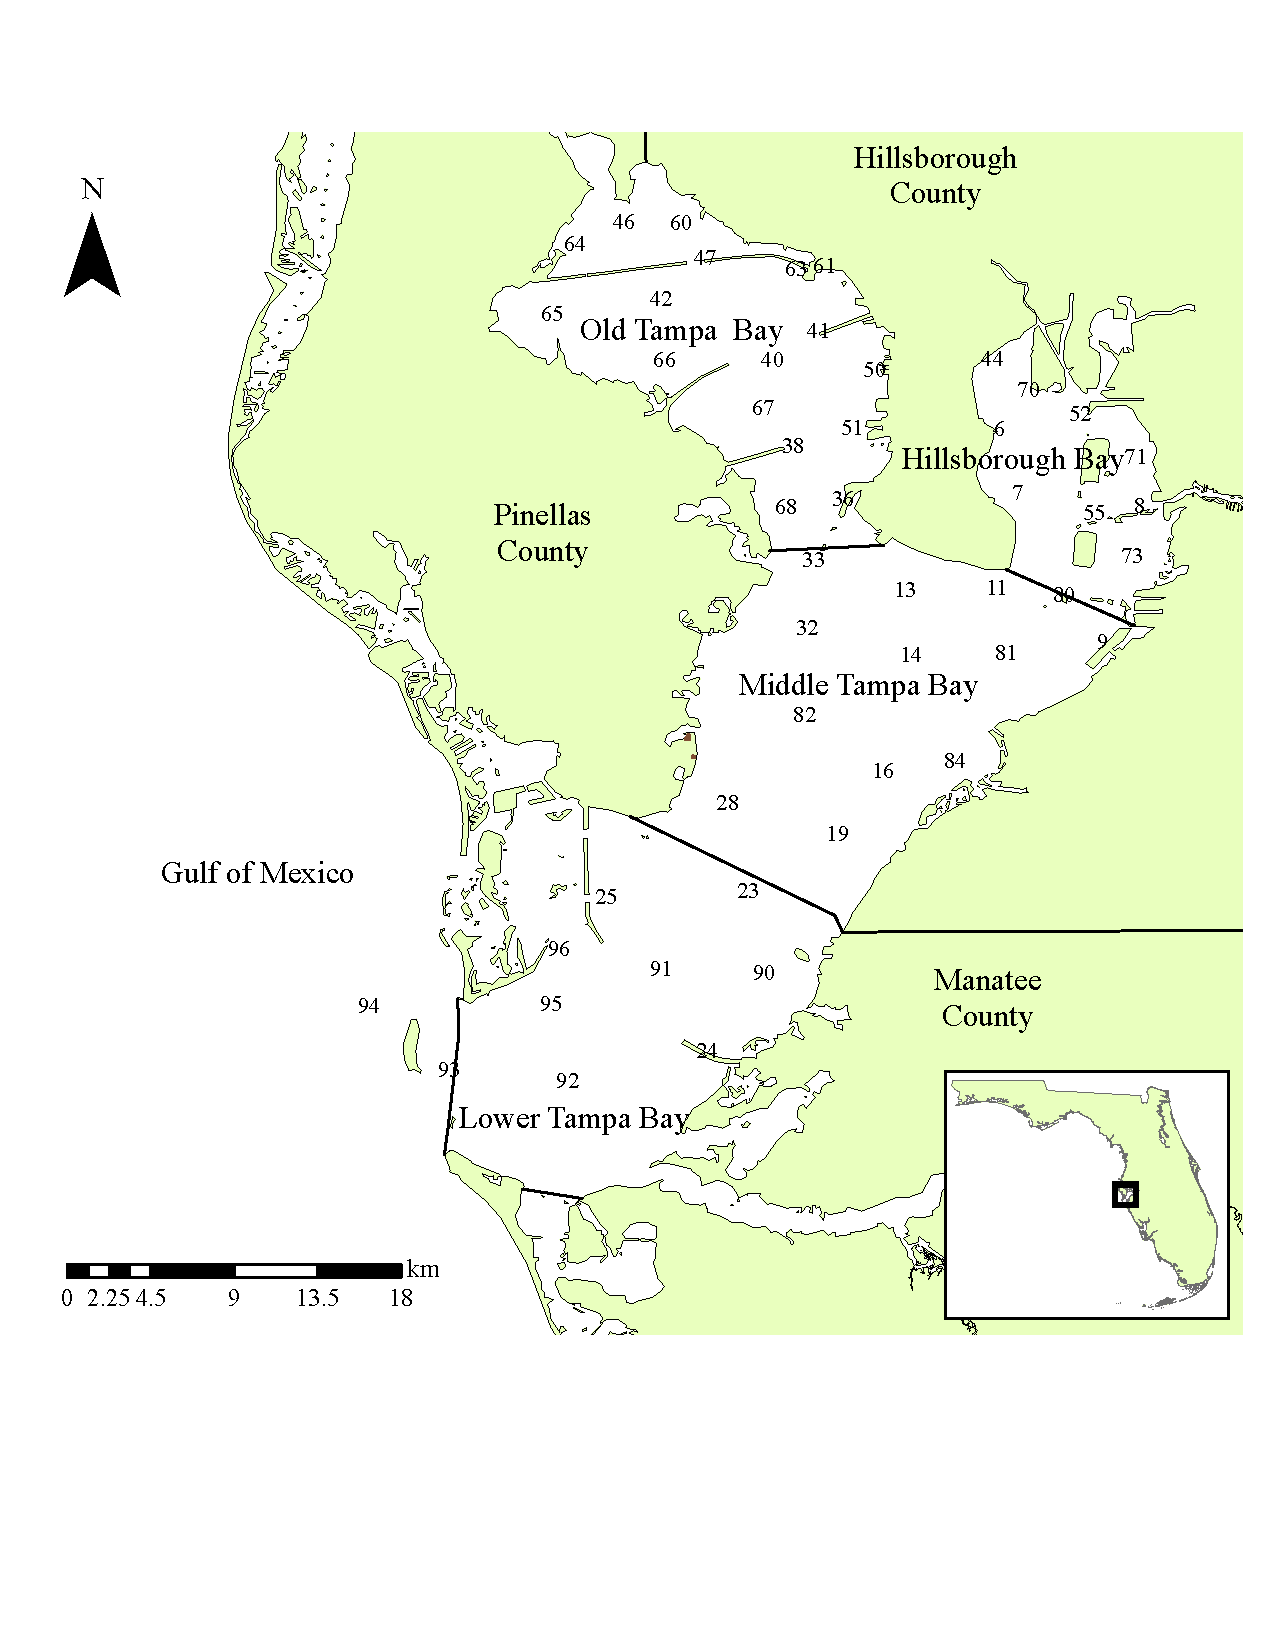
\includegraphics[width=0.9\textwidth]{M:/docs/manuscripts/tb_chl/figs/tb_map.pdf}
\caption{The Tampa Bay estuary located on the west coast of central Florida. The Bay is separated into four segments defined by chemical, physical, and geopolitical boundaries \cite{Lewis85}. Monthly water quality monitoring stations are also indicated by their identification number \cite{Boler01}.}
\label{fig:tb_map}
\end{figure}

%obs chlorophyll by year/month, uses station data

\begin{figure}
\centering
\subfloat[By year]{
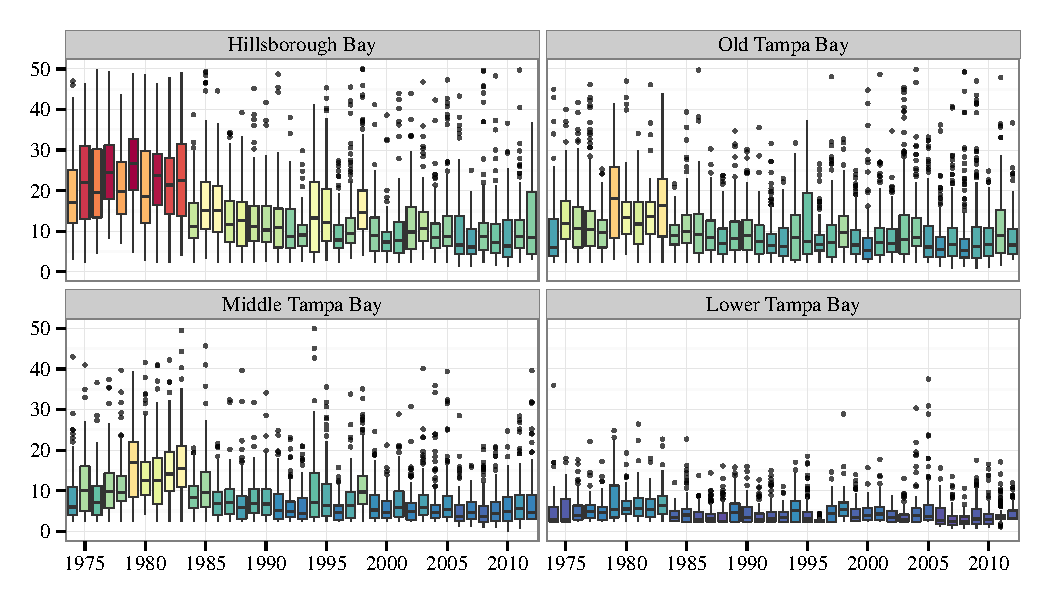
\includegraphics[width=\textwidth,page=1]{M:/docs/manuscripts/tb_chl/figs/obsyrmo.pdf}
\label{fig:obsyrmo1}
}

\subfloat[By month]{
\includegraphics[width=\textwidth,page=2]{M:/docs/manuscripts/tb_chl/figs/obsyrmo.pdf}
\label{fig:obsyrmo2}
}

\leavevmode\smash{\makebox[0pt]{\hspace{0em}% HORIZONTAL POSITION           
  \rotatebox[origin=l]{90}{\hspace{19em}% VERTICAL POSITION
    Chlorophyll-\textit{a} (\mugl)}%
}}\hspace{0pt plus 1filll}\null

\caption{Observed \ac{chl} data for Tampa Bay segments by \protect\subref{fig:obsyrmo1} year and \protect\subref{fig:obsyrmo2} month aggregations.  Each box is bisected by the median and represents the \ac{IQR} (25\textsuperscript{th} to 75\textsuperscript{th} percentile).  Outliers are present beyond whiskers (1.5$\cdot$\ac{IQR}) and were observed beyond 50 \mugl.}
\label{fig:obsyrmo}
\end{figure}

%weighting example
\begin{figure}[!ht]


{\centering 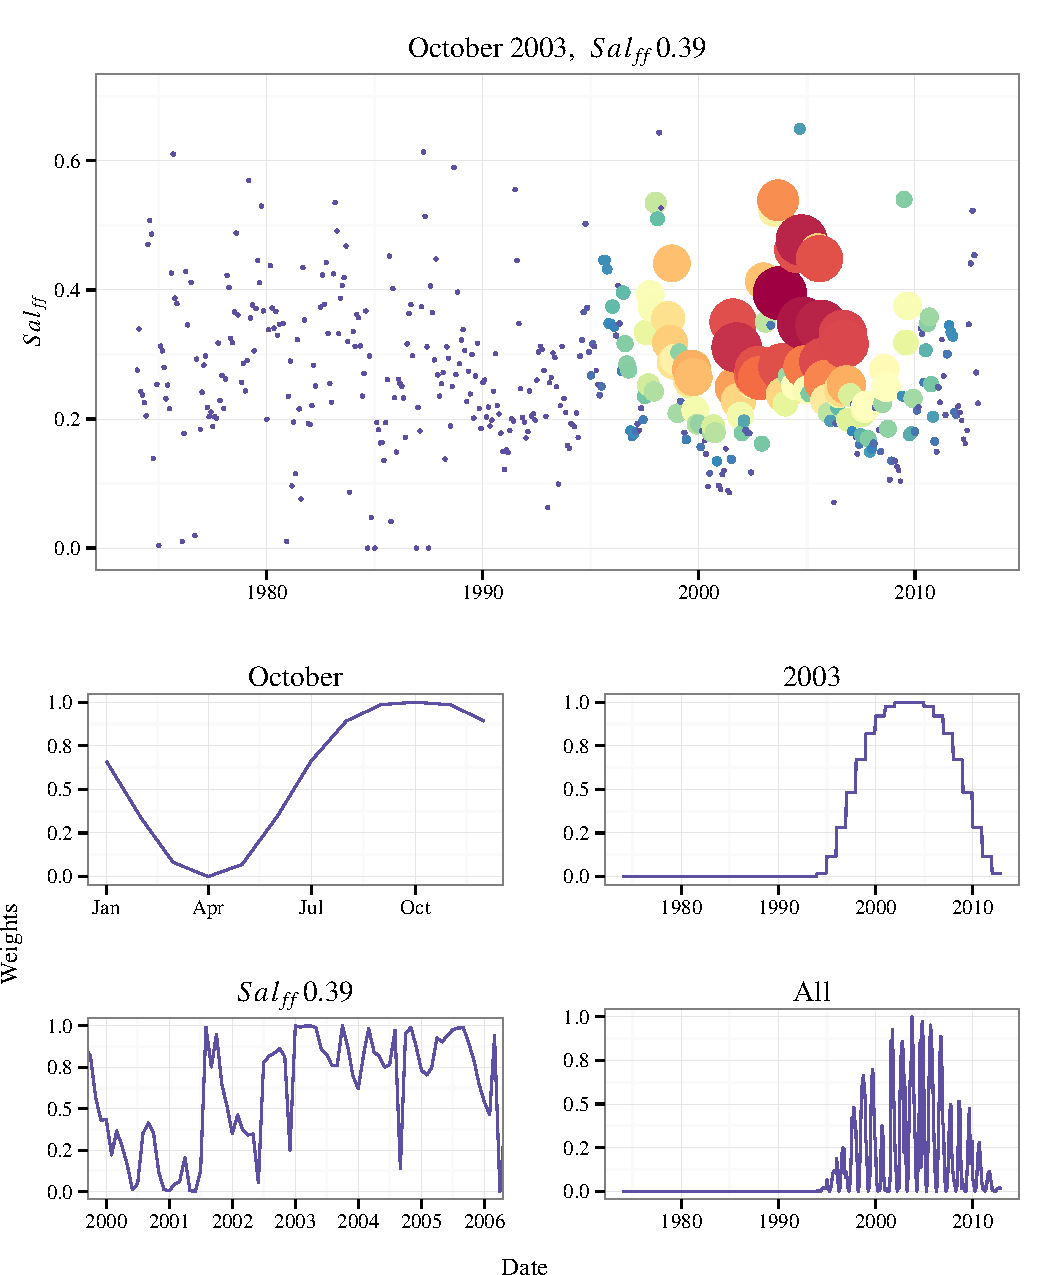
\includegraphics[width=6in]{M:/docs/manuscripts/tb_chl/figs/wtex} 

}

\caption[Example of weighting for one observation in Hillsborough Bay]{Example of weighting for one observation in Hillsborough Bay.  The top plot shows all data weighted for October 2003 when the proportion freshwater was 0.39.  Point size and color are in proportion to weights (small grey points = 0, large black points = 1).  The bottom plots show the individual weights for month, year, proportion freshwater, and all weights combined.\label{fig:wtex}}
\end{figure}



%predictions from model, all data
\begin{figure}[!ht]


{\centering 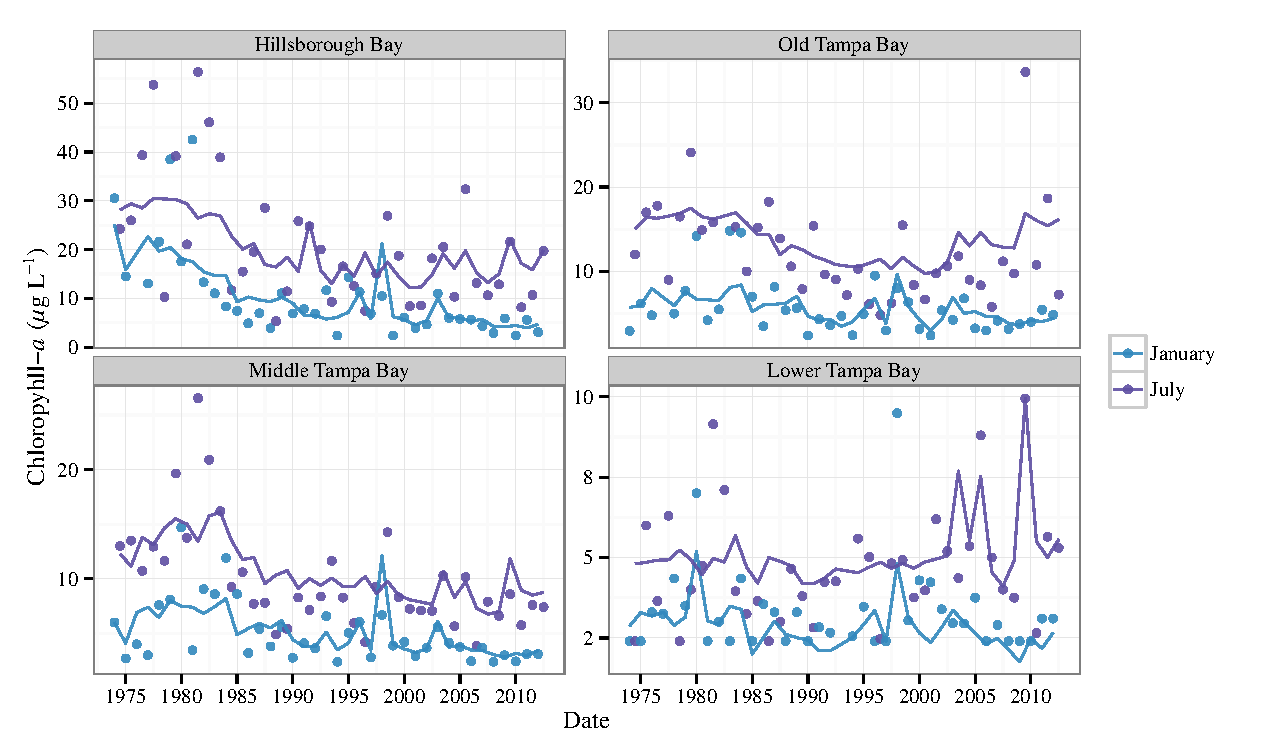
\includegraphics[width=6in]{M:/docs/manuscripts/tb_chl/figs/predobs} 

}

\caption[Predicted (lines) and observed (circles) \ac{chl} concentrations for Tampa Bay segments in January (dry season) and July (wet season) (see supplements for all months)]{Predicted (lines) and observed (circles) \ac{chl} concentrations for Tampa Bay segments in January (dry season) and July (wet season) (see supplements for all months).  Predicted values are for the weighted regression models fit through the mean response.\label{fig:predobs}}
\end{figure}



\begin{figure}[!ht]


{\centering 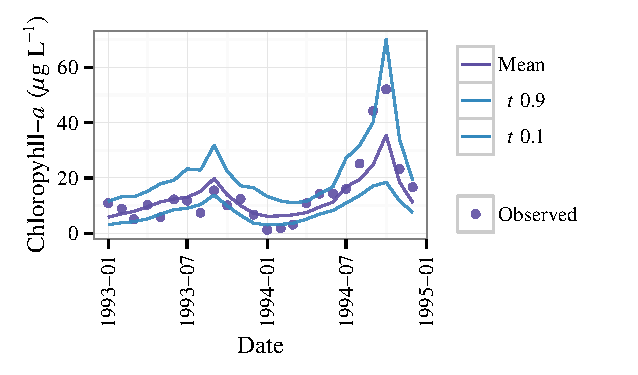
\includegraphics[width=3in]{M:/docs/manuscripts/tb_chl/figs/hbslice} 

}

\caption[Predicted and observed \ac{chl} concentrations for Hillsborough Bay for 1993 to 1995 illustrating variation in model fit based on observation date]{Predicted and observed \ac{chl} concentrations for Hillsborough Bay for 1993 to 1995 illustrating variation in model fit based on observation date. Predicted values are for the weighted regression models fit through the mean response and the 10\textsuperscript{th} and 90\textsuperscript{th} percentile ($\tau$) distributions.\label{fig:hbslice}}
\end{figure}



\begin{figure}[!ht]


{\centering 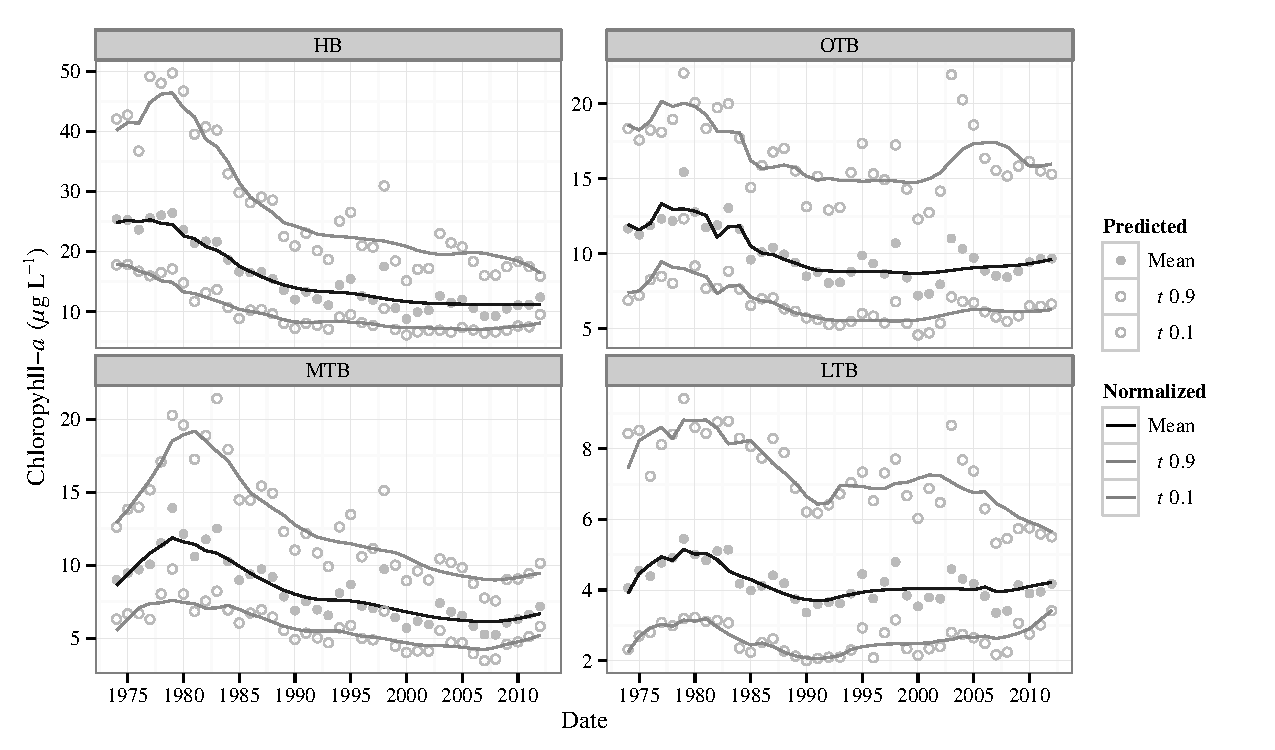
\includegraphics[width=6in]{M:/docs/manuscripts/tb_chl/figs/salnrm} 

}

\caption[Weighted regression predictions and salinity-normalized results aggregated by year for the mean response and the 10\textsuperscript{th} and 90\textsuperscript{th} quantile ($\tau$) distributions]{Weighted regression predictions and salinity-normalized results aggregated by year for the mean response and the 10\textsuperscript{th} and 90\textsuperscript{th} quantile ($\tau$) distributions.\label{fig:salnrm}}
\end{figure}



\begin{figure}[!ht]


{\centering 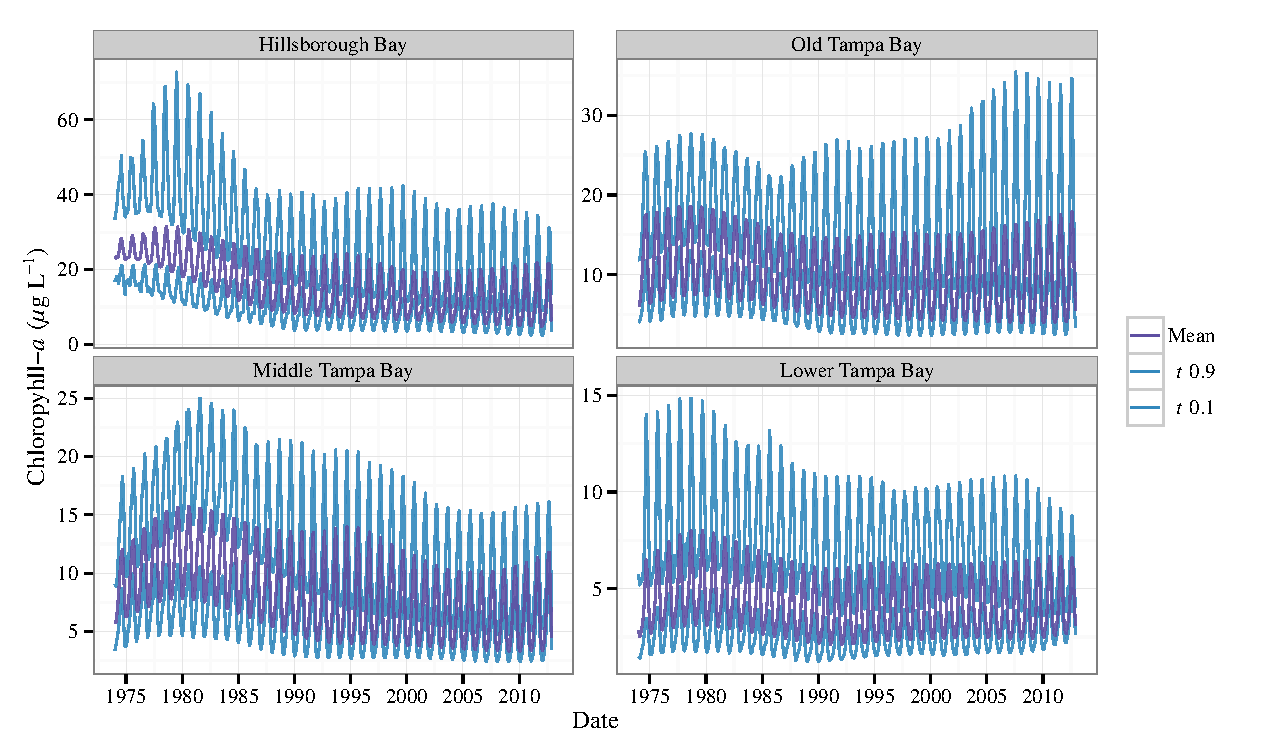
\includegraphics[width=6in]{M:/docs/manuscripts/tb_chl/figs/salnrm2} 

}

\caption[Salinity-normalized results for the mean response and the 10\textsuperscript{th} and 90\textsuperscript{th} quantile ($\tau$) distributions]{Salinity-normalized results for the mean response and the 10\textsuperscript{th} and 90\textsuperscript{th} quantile ($\tau$) distributions. Note changes in intra-annual variability by bay segment.\label{fig:salnrm2}}
\end{figure}



\begin{figure}[!ht]


{\centering 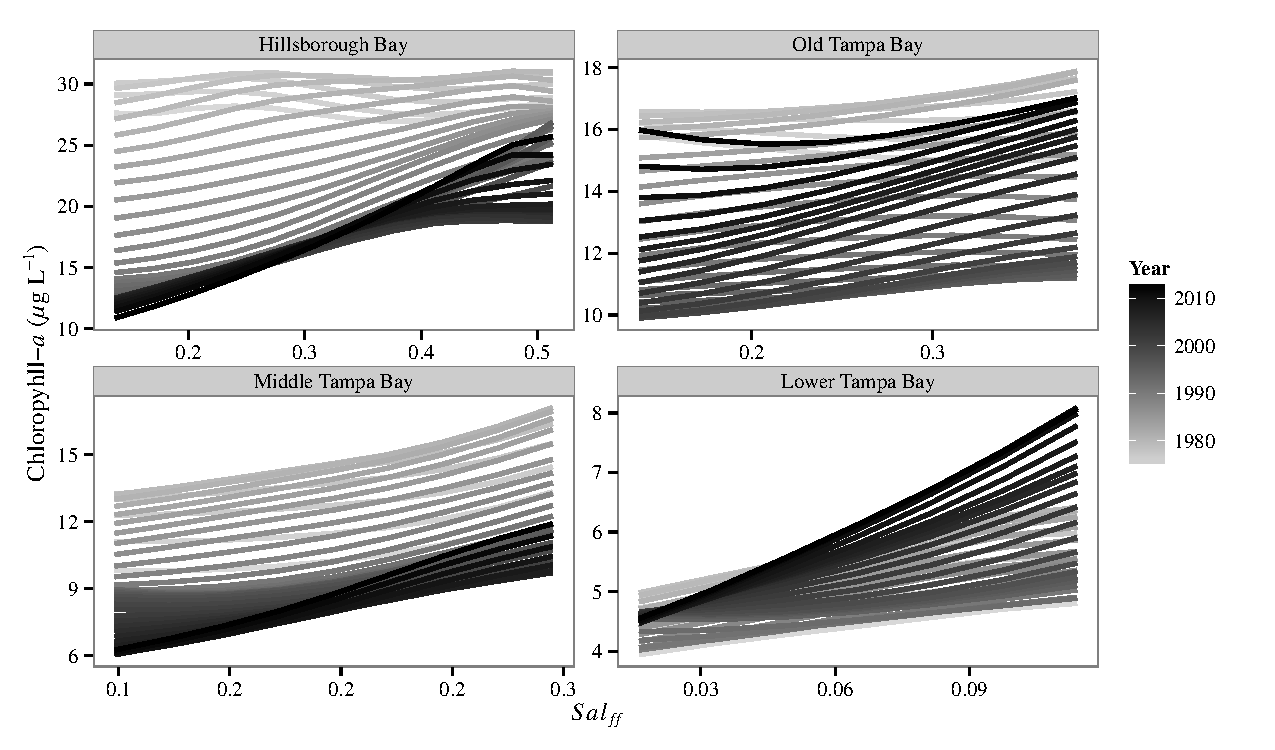
\includegraphics[width=6in]{M:/docs/manuscripts/tb_chl/figs/dyna} 

}

\caption[Variation in the relationship between \ac{chl} and salinity as fraction of freshwater ($Sal_{ff}$) across time series for Tampa Bay]{Variation in the relationship between \ac{chl} and salinity as fraction of freshwater ($Sal_{ff}$) across time series for Tampa Bay. Data are for July months to reduce seasonal variation. Only the mean response models are shown.\label{fig:dyna}}
\end{figure}



\beginsupplement
%predictions from model, all data
\begin{landscape}
\centering\vspace*{\fill}
\begin{figure}[!ht]


{\centering 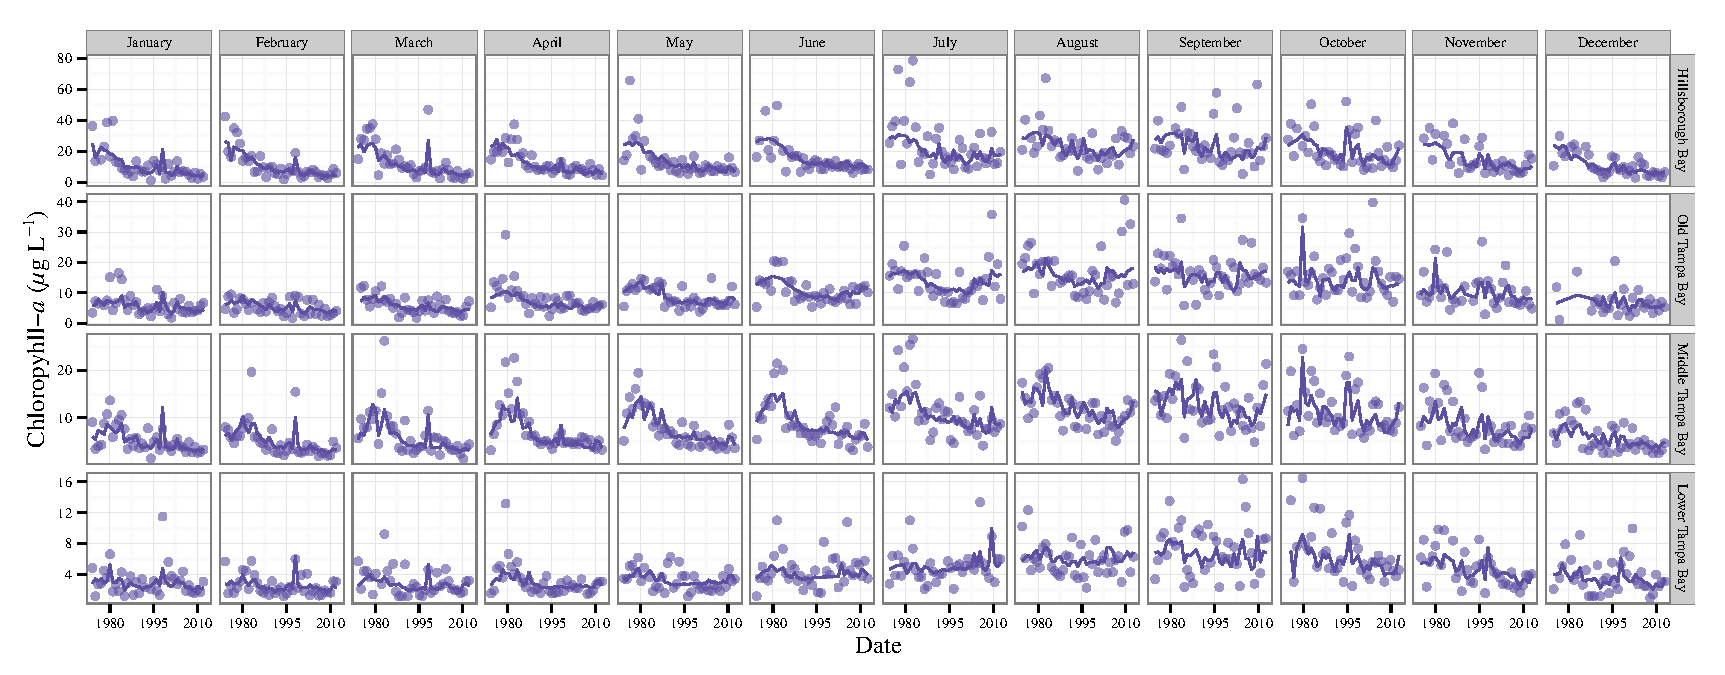
\includegraphics[width=9in]{M:/docs/manuscripts/tb_chl/figs/sup} 

}

\caption[Predicted (lines) and observed (circles) \ac{chl} concentrations for Tampa Bay segments by month]{Predicted (lines) and observed (circles) \ac{chl} concentrations for Tampa Bay segments by month.  Predicted values are for the weighted regression models fit through the mean response.\label{fig:sup}}
\end{figure}


\vfill
\end{landscape}

\end{document}
